\documentclass[a4paper,12pt]{article}

\usepackage[T2A]{fontenc}			
\usepackage[utf8]{inputenc}			
\usepackage[english,russian]{babel}	

\usepackage[
bookmarks=true, colorlinks=true, unicode=true,
urlcolor=black,linkcolor=black, anchorcolor=black,
citecolor=black, menucolor=black, filecolor=black,
]{hyperref}

\usepackage{color}
\usepackage{caption}
\DeclareCaptionFont{white}{\color{black}}
\DeclareCaptionFormat{listing}{\colorbox{white}{\parbox{\textwidth}{#1#2#3}}}
\captionsetup[lstlisting]{format=listing,labelfont=white,textfont=white}

\usepackage{amsmath,amsfonts,amssymb,amsthm,mathtools} 
\usepackage{wasysym}

\usepackage{graphicx}
%\usepackage[cache=false]{minted}
\usepackage{cmap}
\usepackage{indentfirst}

\usepackage{listings} 
\usepackage{fancyvrb}

\usepackage{geometry}
\geometry{left=2cm}
\geometry{right=1.5cm}
\geometry{top=1cm}
\geometry{bottom=2cm}

\setlength{\parindent}{5ex}
\setlength{\parskip}{0.5em}

\usepackage{pgfplots}

\usepackage{longtable}

\begin{document}
	\lstset{ %
		language=C,                 % выбор языка для подсветки (здесь это С)
		basicstyle=\small\sffamily, % размер и начертание шрифта для подсветки кода
		numbers=left,               % где поставить нумерацию строк (слева\справа)
		numberstyle=\tiny,           % размер шрифта для номеров строк
		stepnumber=1,                   % размер шага между двумя номерами строк
		numbersep=5pt,                % как далеко отстоят номера строк от подсвечиваемого кода
		backgroundcolor=\color{white}, % цвет фона подсветки - используем \usepackage{color}
		showspaces=false,            % показывать или нет пробелы специальными отступами
		showstringspaces=false,      % показывать или нет пробелы в строках
		showtabs=false,             % показывать или нет табуляцию в строках
		frame=single,              % рисовать рамку вокруг кода
		tabsize=2,                 % размер табуляции по умолчанию равен 2 пробелам
		captionpos=t,              % позиция заголовка вверху [t] или внизу [b] 
		breaklines=true,           % автоматически переносить строки (да\нет)
		breakatwhitespace=false, % переносить строки только если есть пробел
		escapeinside={\%*}{*)}   % если нужно добавить комментарии в коде
	}
	
	% Титульный лист
	\begin{figure}[h!]
		\begin{center}
			{
\includegraphics[scale = 0.4]{titul.jpg}}
			\label{titul}
		\end{center}
	\end{figure}
	
	\vspace*{15mm} 
	
	\huge
	\begin{center}
		Дисциплина: <<Компьютерные сети>>
	\end{center}
	
	\begin{center}
		Лабораторная работа №4
	\end{center}

	
	\huge
	\begin{center}
		Вариант 7
	\end{center}
	\vspace*{25mm} 
	
	\large
	\begin{flushright}
		Студент: Левушкин И. К. \\
		Группа: ИУ7-72Б \\
		Преподаватель: Рудаков И. В. \\
	\end{flushright}
	
	\vspace*{25mm}
	\begin{center}
		Москва, 2020 г.  
	\end{center}
	\thispagestyle{empty}
	
	
	\newpage
	
	\section{Присвоить портам устройств статические ipv4 адреса в соответствии с вариантом. Адрес устройства определяется по формулам ниже ($x = 7,  y$ – порядковый номер от 1 и выше).}
	
	\begin{itemize}
		\item Адрес ПК (сеть 1): 10.1.7.1 255.255.255.0
		\item Адрес DNS-сервера (сеть 2): 192.168.7.1 255.255.255.0
		\item Адрес HTTP- и SMTP-серверов (сеть 3): 172.16.7.1 255.255.255.0 и 172.16.7.2 255.255.255.0
	\end{itemize}

	\begin{figure}[h!]
		\begin{minipage}[b]{0.32\textwidth}
			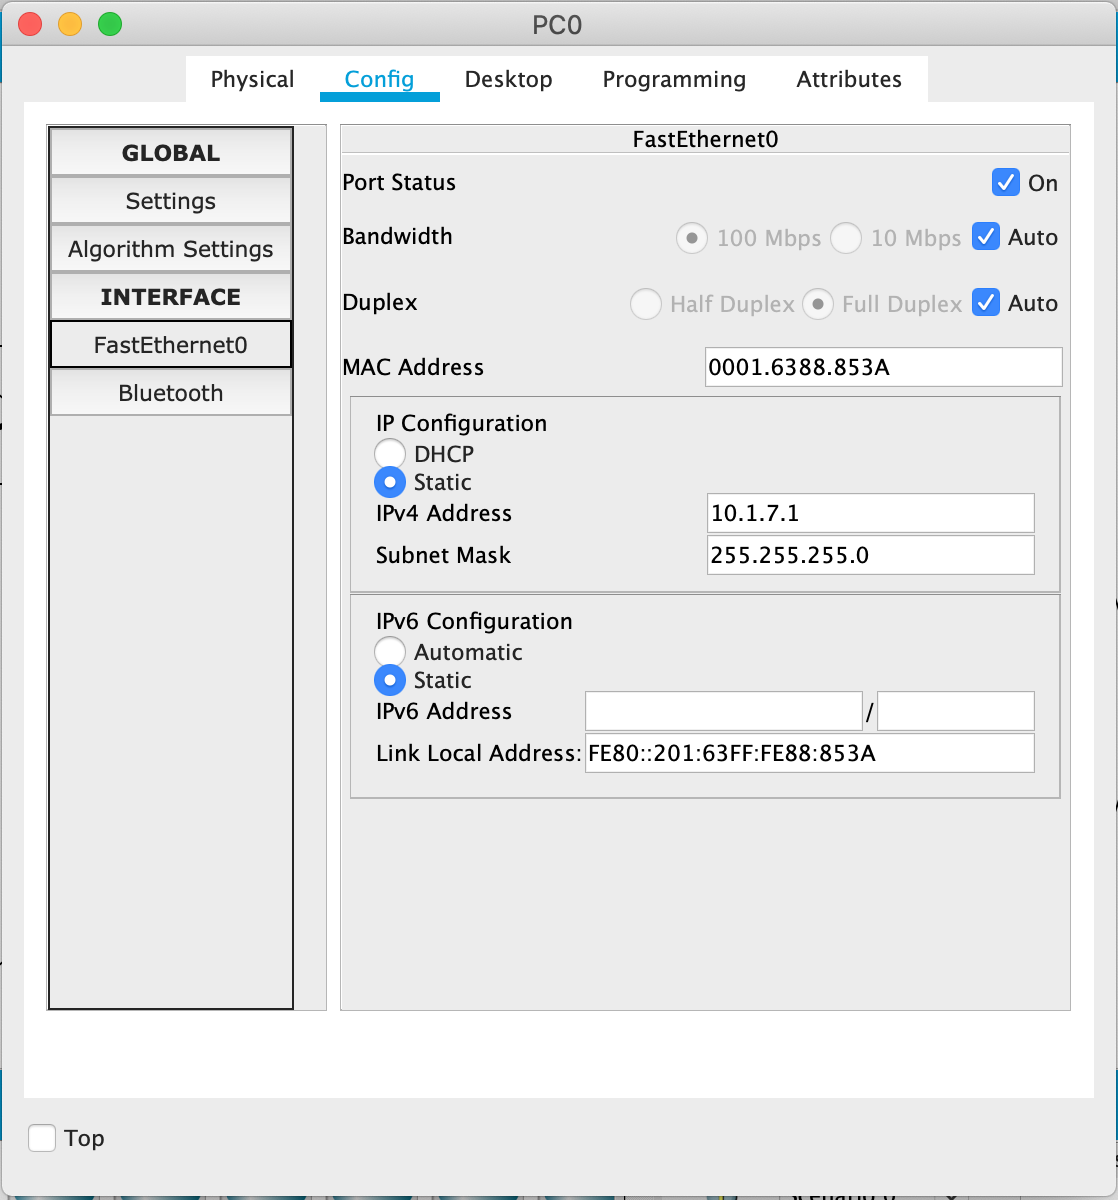
\includegraphics[width=\textwidth]{1.1.png}
		\end{minipage}
		\begin{minipage}[b]{0.32\textwidth}
			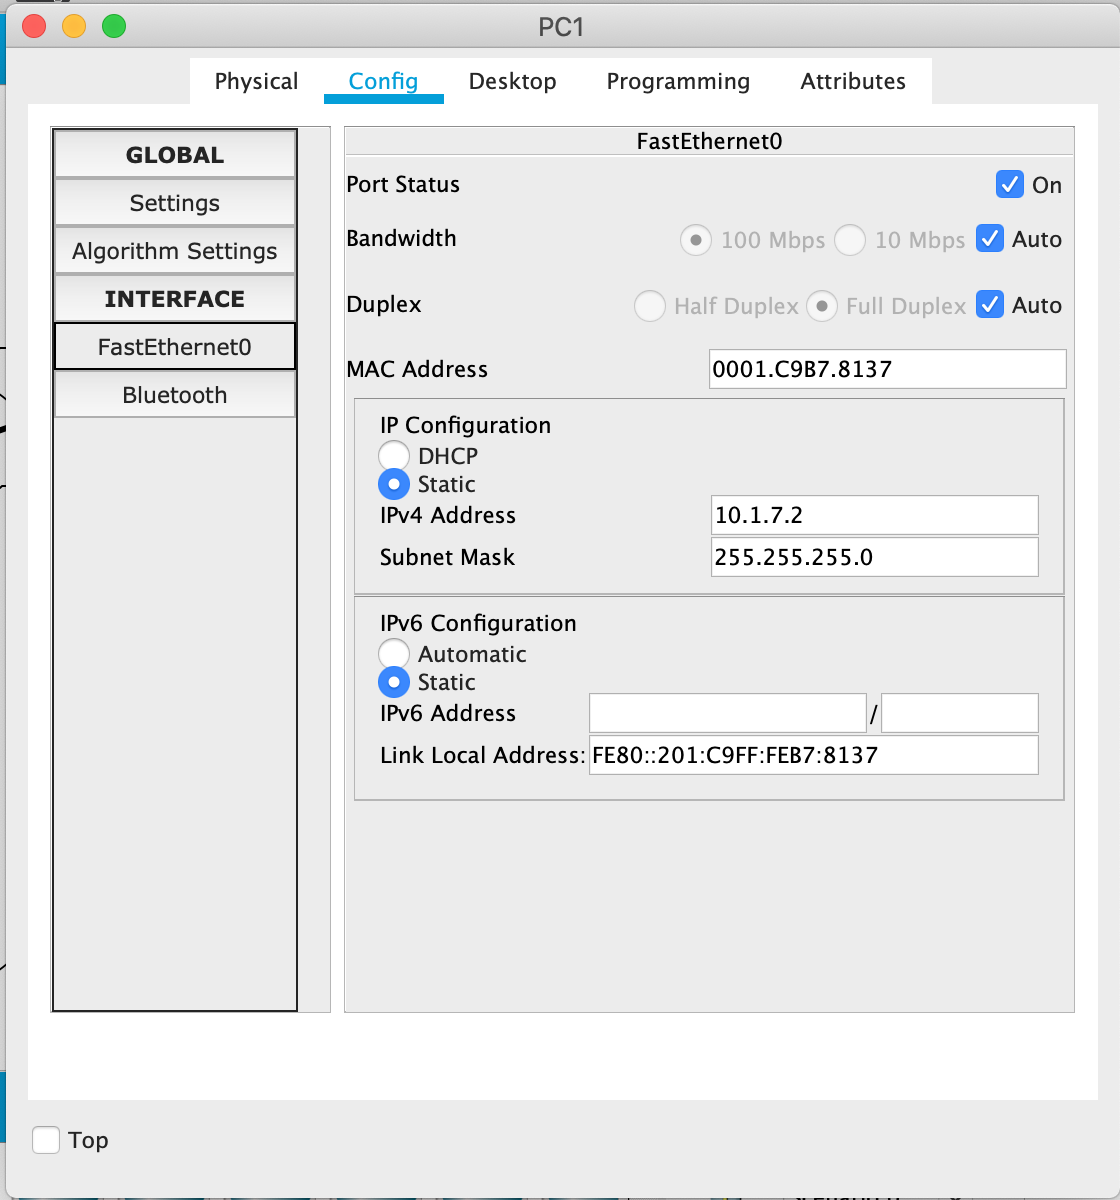
\includegraphics[width=\textwidth]{1.2.png}
		\end{minipage}
		\begin{minipage}[b]{0.32\textwidth}
			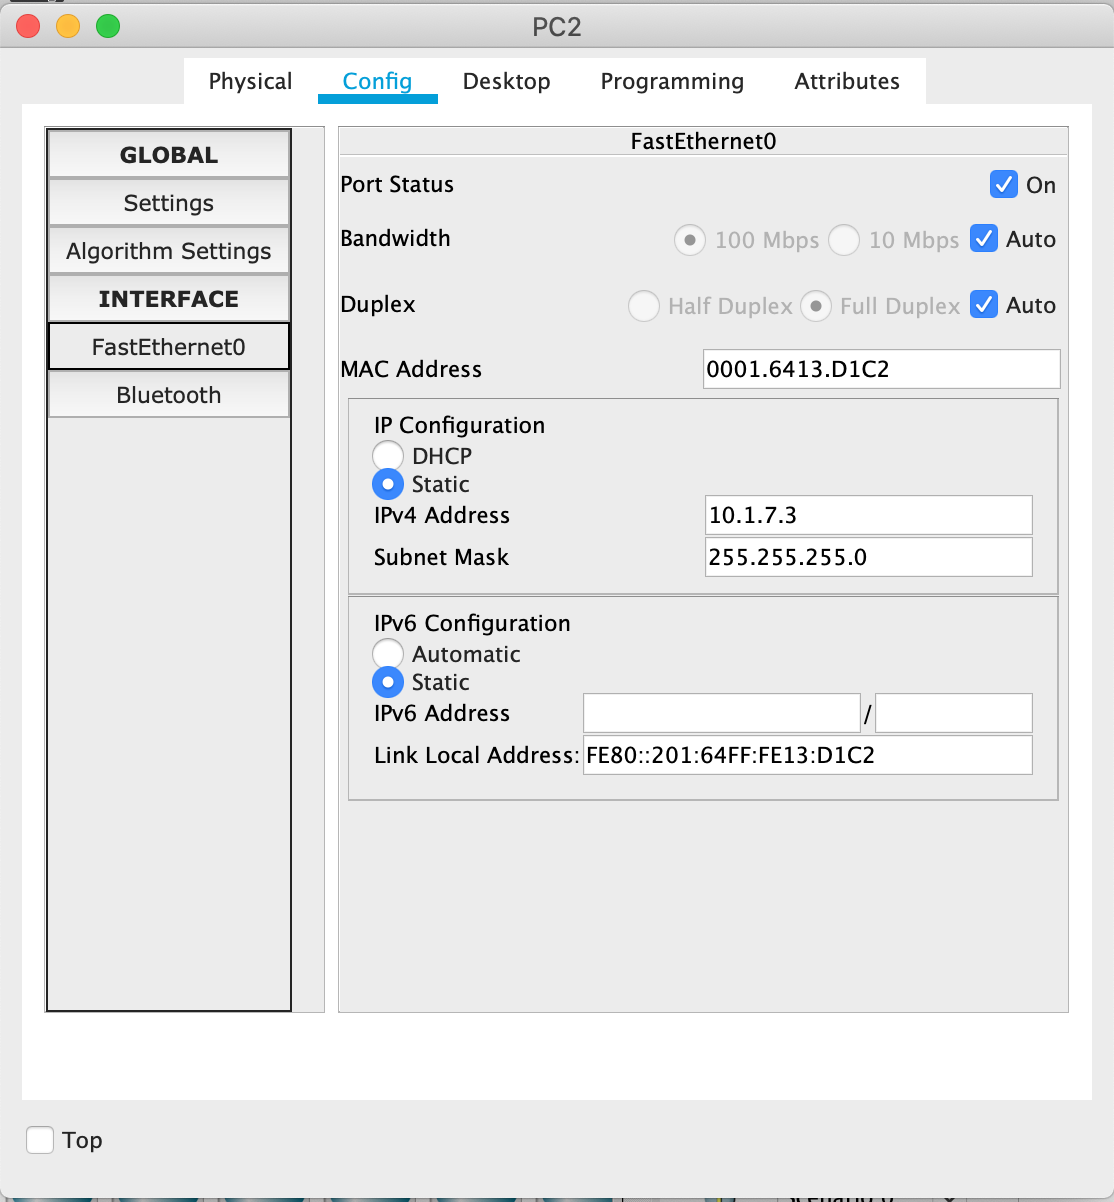
\includegraphics[width=\textwidth]{1.3.png}
		\end{minipage}
		\center{Установка адресов для ПК}
		\label{ris:1}
	\end{figure}
	
	\begin{figure}[h!]
		\begin{minipage}[b]{0.32\textwidth}
			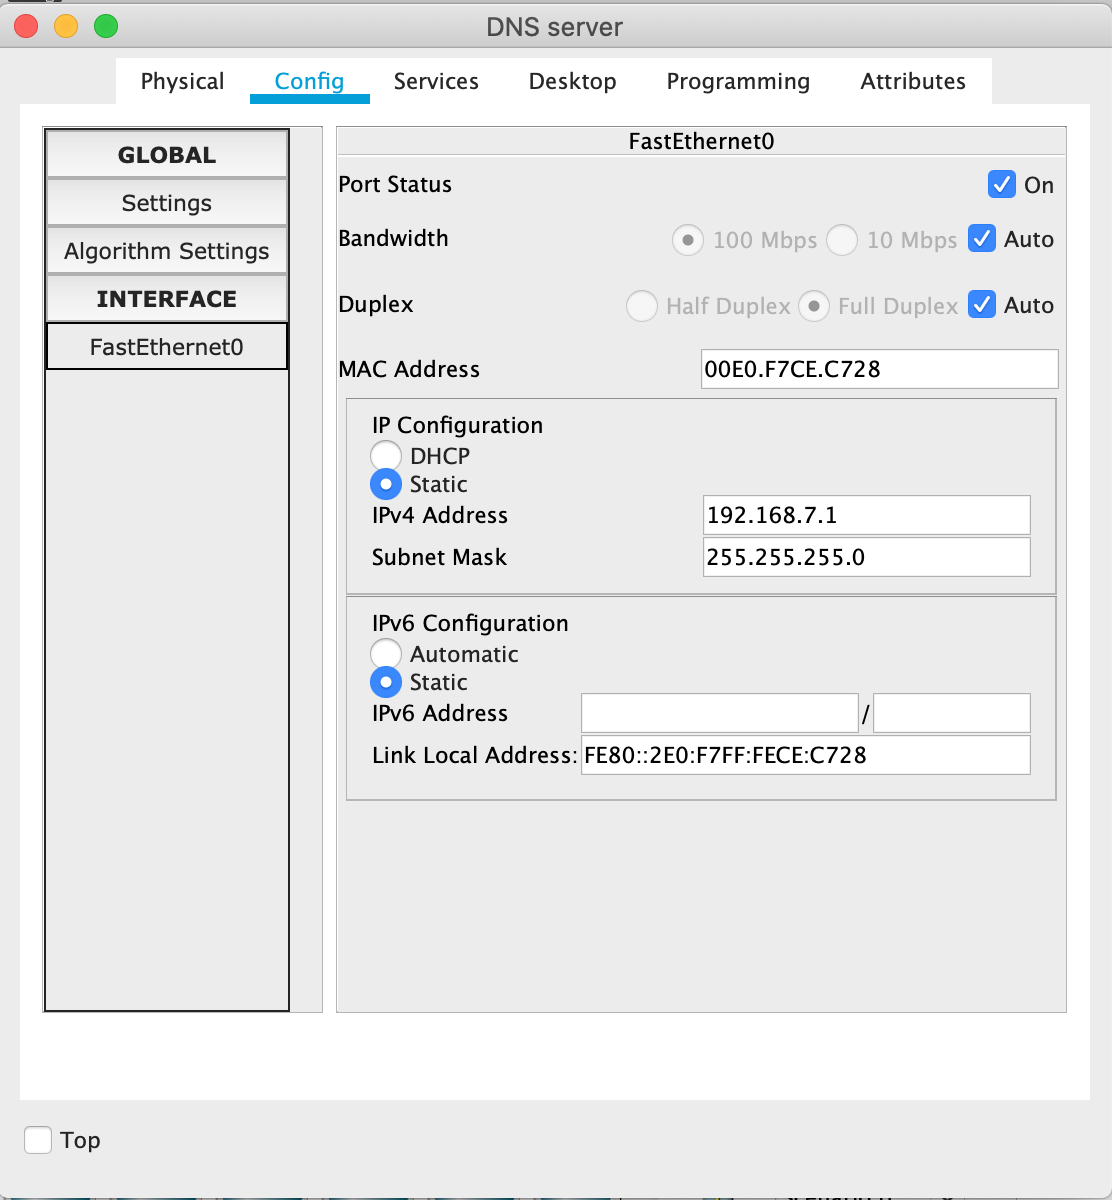
\includegraphics[width=\textwidth]{2.1.png}
			\center{Установка адреса для DNS-сервера}
		\end{minipage}
		\begin{minipage}[b]{0.32\textwidth}
			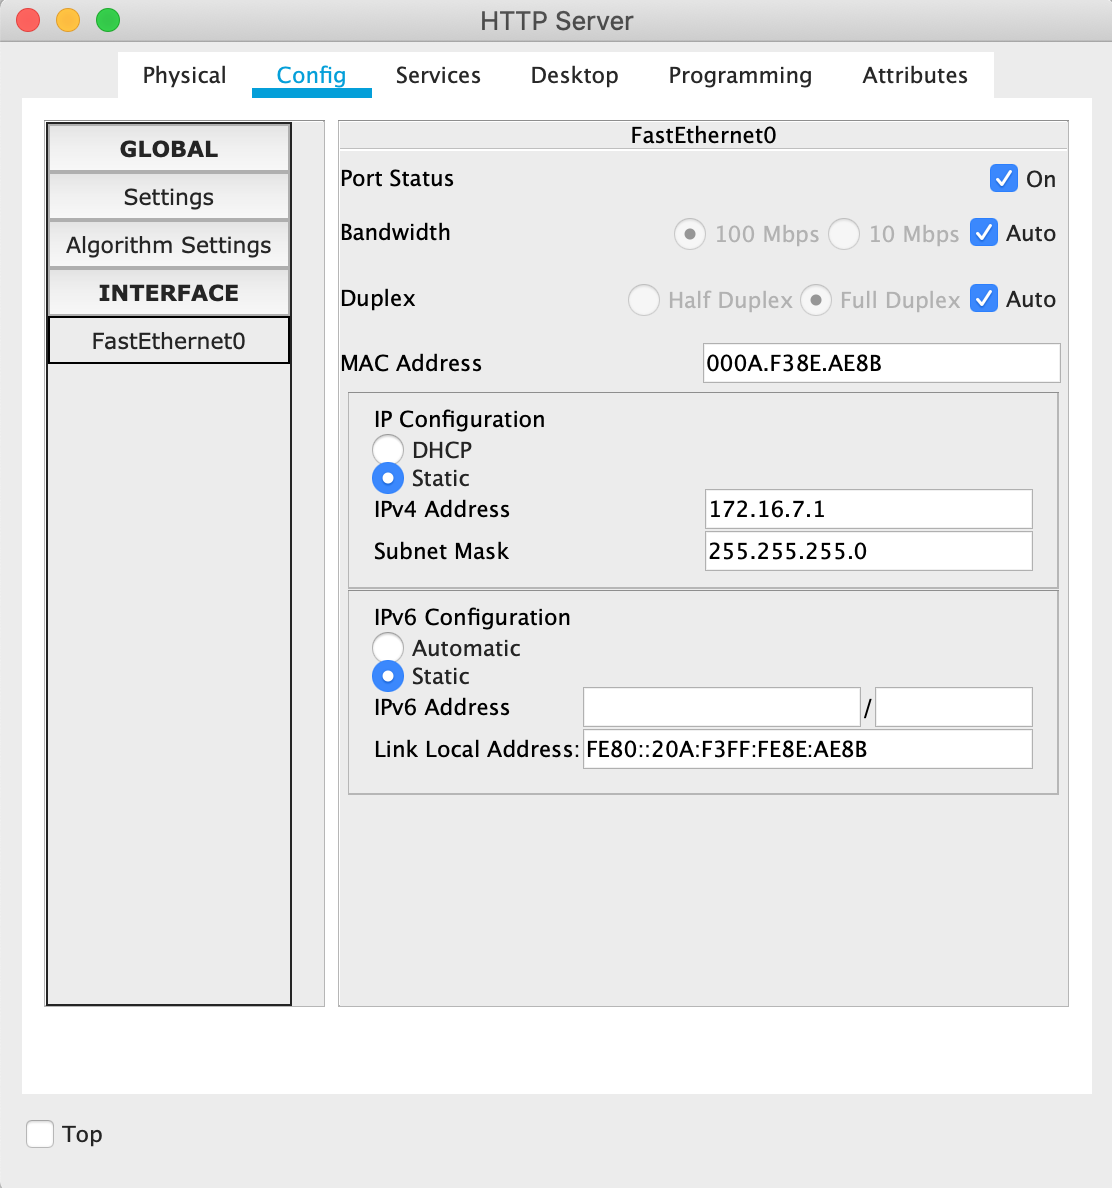
\includegraphics[width=\textwidth]{2.2.png}
			\center{Установка адреса для HTTP-сервера}
		\end{minipage}
		\begin{minipage}[b]{0.32\textwidth}
			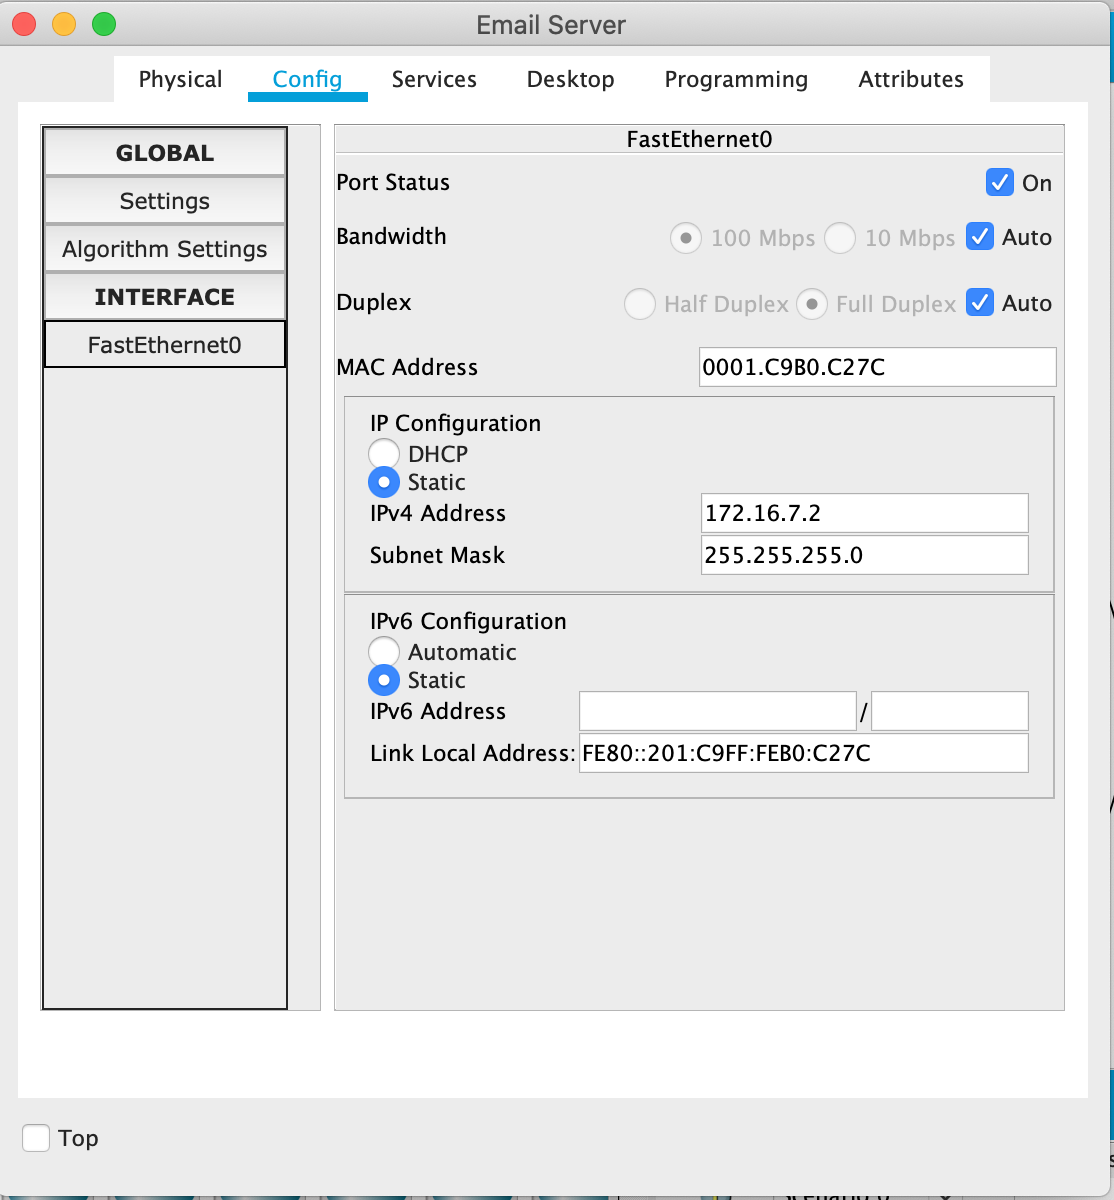
\includegraphics[width=\textwidth]{2.3.png}
			\center{Установка адреса для SMTP-сервера}
		\end{minipage}
		\label{ris:2}
	\end{figure}

	\newpage
	
	\section{Настроить безопасный доступ к коммутаторам и маршрутизатору.}
	
	\begin{figure}[h!]
		\begin{center}
			{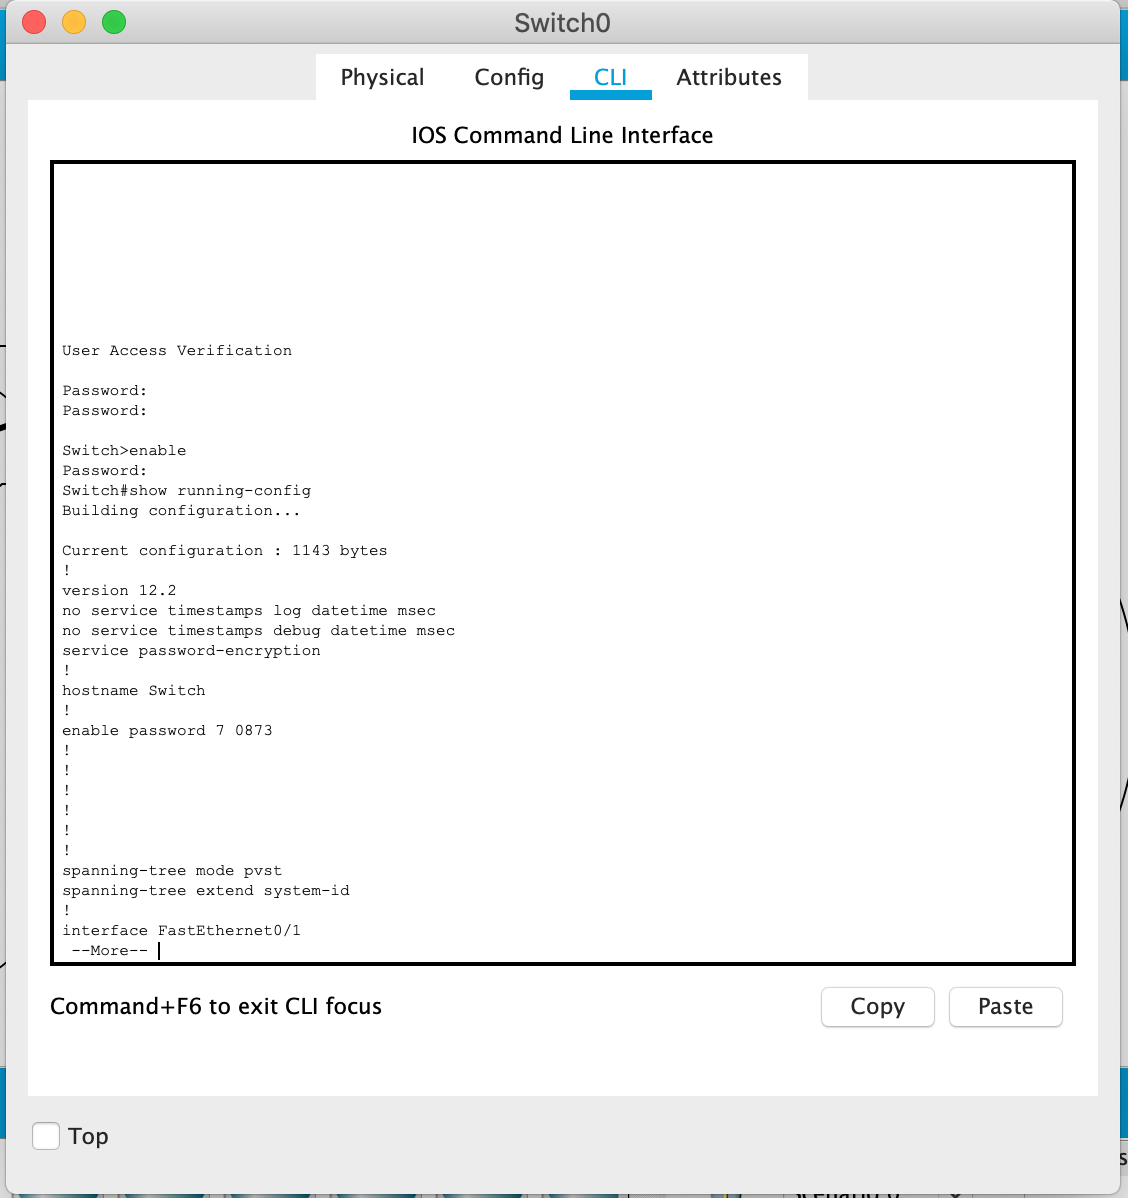
\includegraphics[scale = 0.6]{3.png}}
			\label{ris:3}
		\end{center}
		\caption{Просмотр настроек при безопасном доступе на примере коммутатора.}
	\end{figure}

	\newpage
	
	\section{Указать адреса портов маршрутизатора как адрес шлюза по умолчанию для конечных узлов. Указать адрес DNS-сервера для конечных узлов.}
	
	\begin{itemize}
		\item Сеть 1: 10.1.7.254 255.255.255.0
		\item Cеть 2: 192.168.7.254 255.255.255.0
		\item Сеть 3: 172.16.7.254 255.255.255.0
	\end{itemize}

	\begin{figure}[h!]
		\begin{center}
			{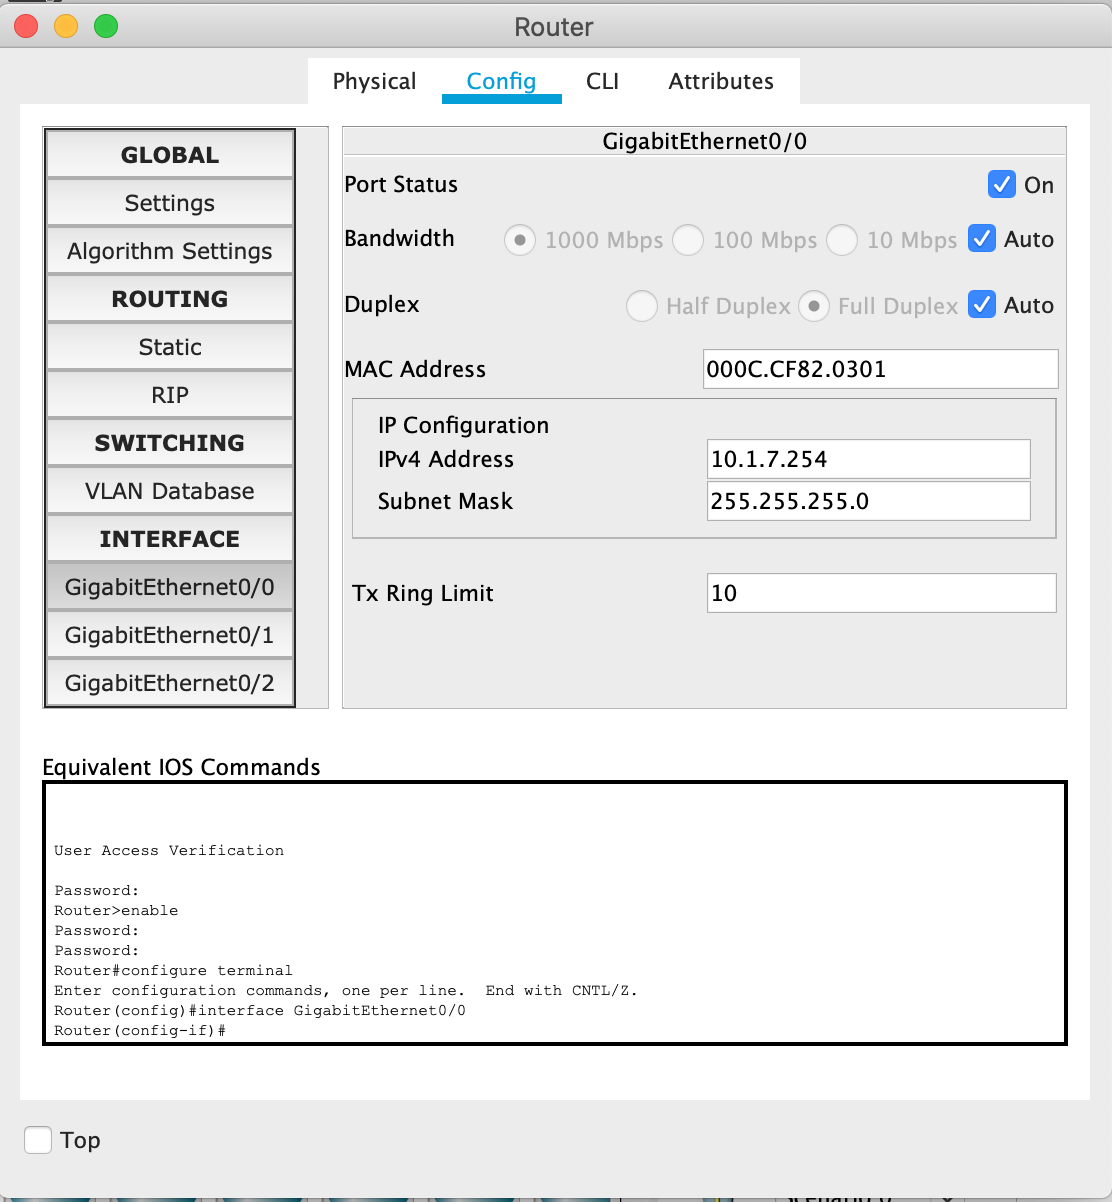
\includegraphics[scale = 0.5]{4.png}}
			\label{ris:4}
		\end{center}
		\caption{Установка портов маршрутизатора как адрес шлюза по умолчанию
			для конечных узлов (сеть 1)}
	\end{figure}


	\begin{figure}[h!]
		\begin{minipage}[b]{0.32\textwidth}
			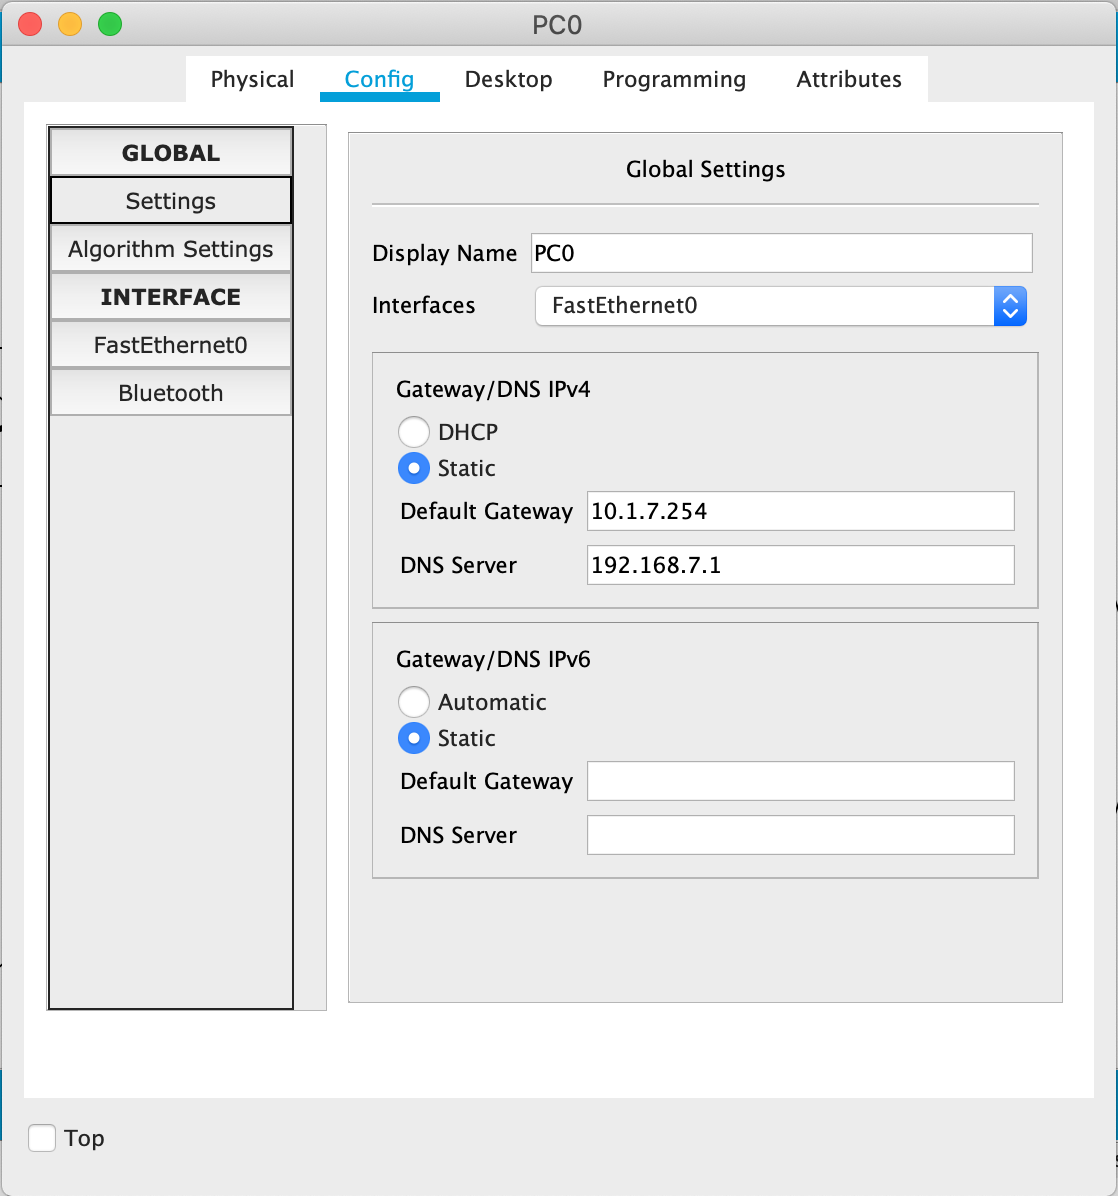
\includegraphics[width=\textwidth]{5.1.png}
		\end{minipage}
		\begin{minipage}[b]{0.32\textwidth}
			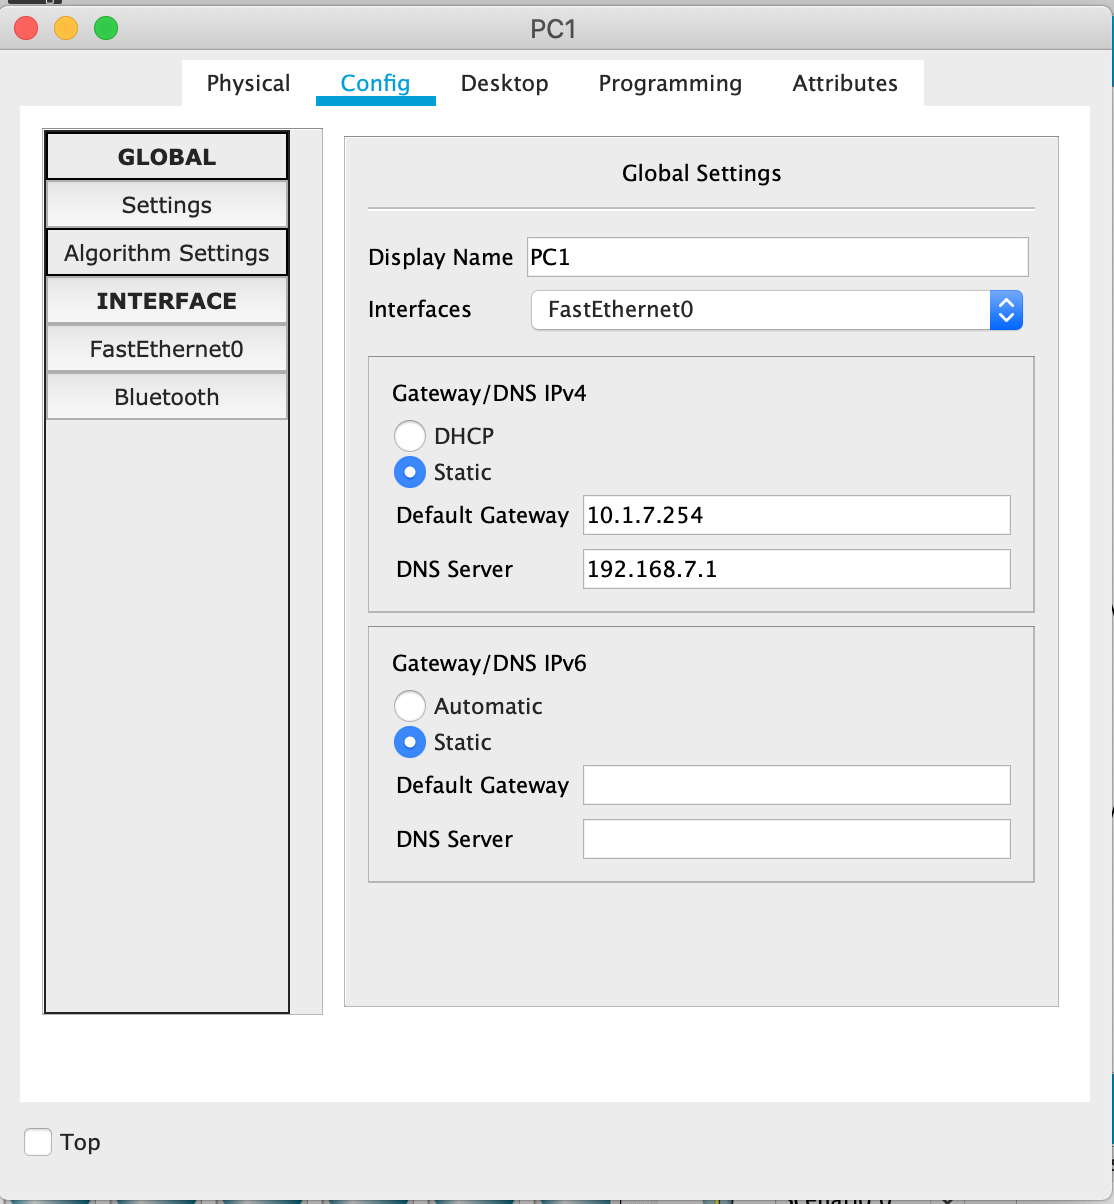
\includegraphics[width=\textwidth]{5.2.png}
		\end{minipage}
		\begin{minipage}[b]{0.32\textwidth}
			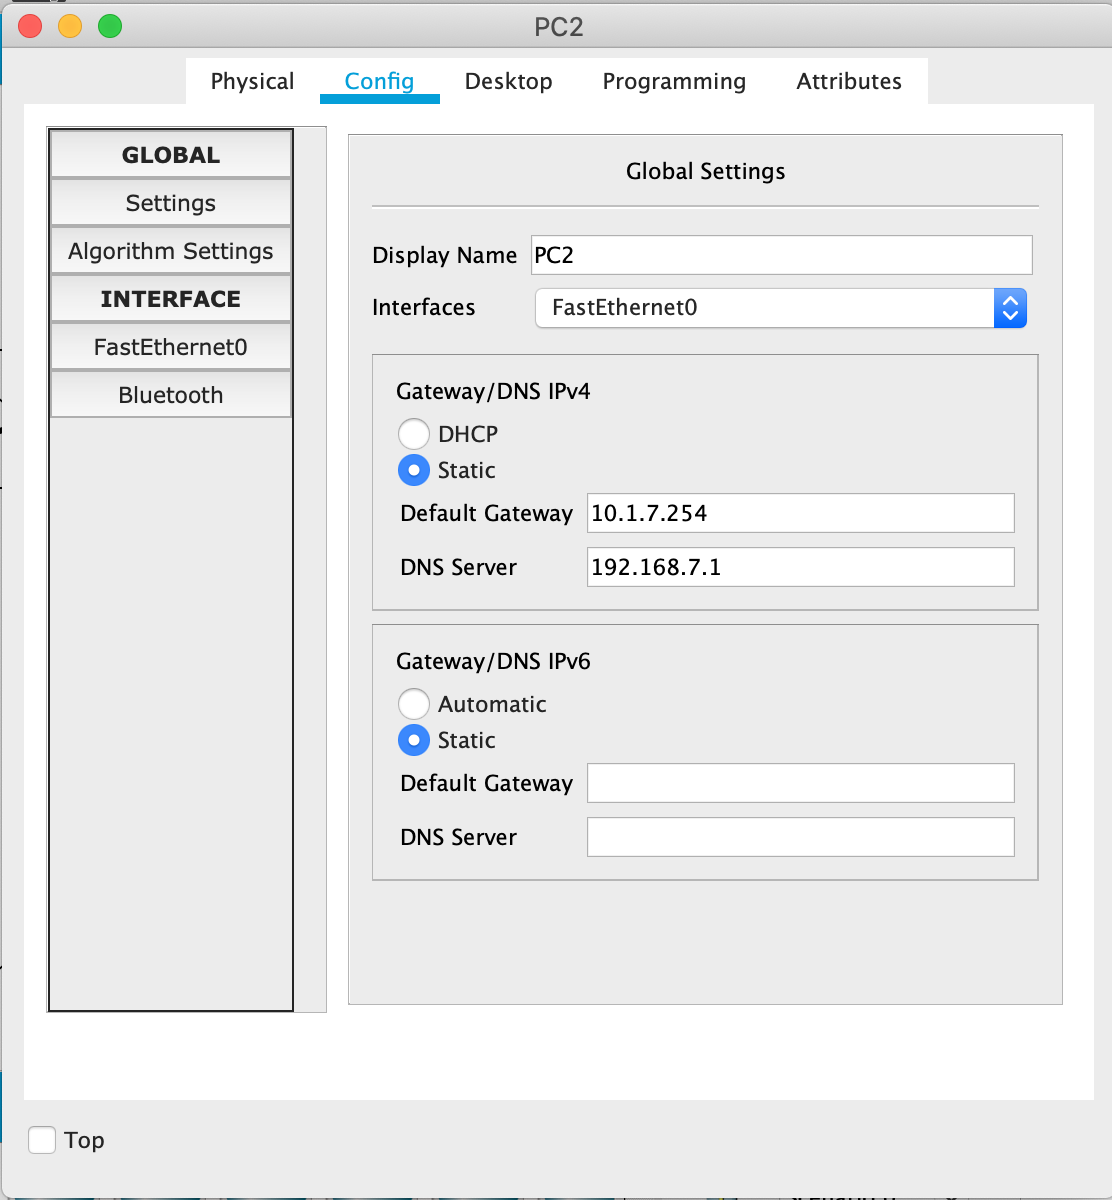
\includegraphics[width=\textwidth]{5.3.png}
		\end{minipage}
		\center{Установка портов маршрутизатора как адрес шлюза по умолчанию
			для конечных узлов (сеть 1)}
		\label{ris:5}
	\end{figure}

	\newpage
	
	\begin{figure}[h!]
		\begin{minipage}[b]{0.32\textwidth}
			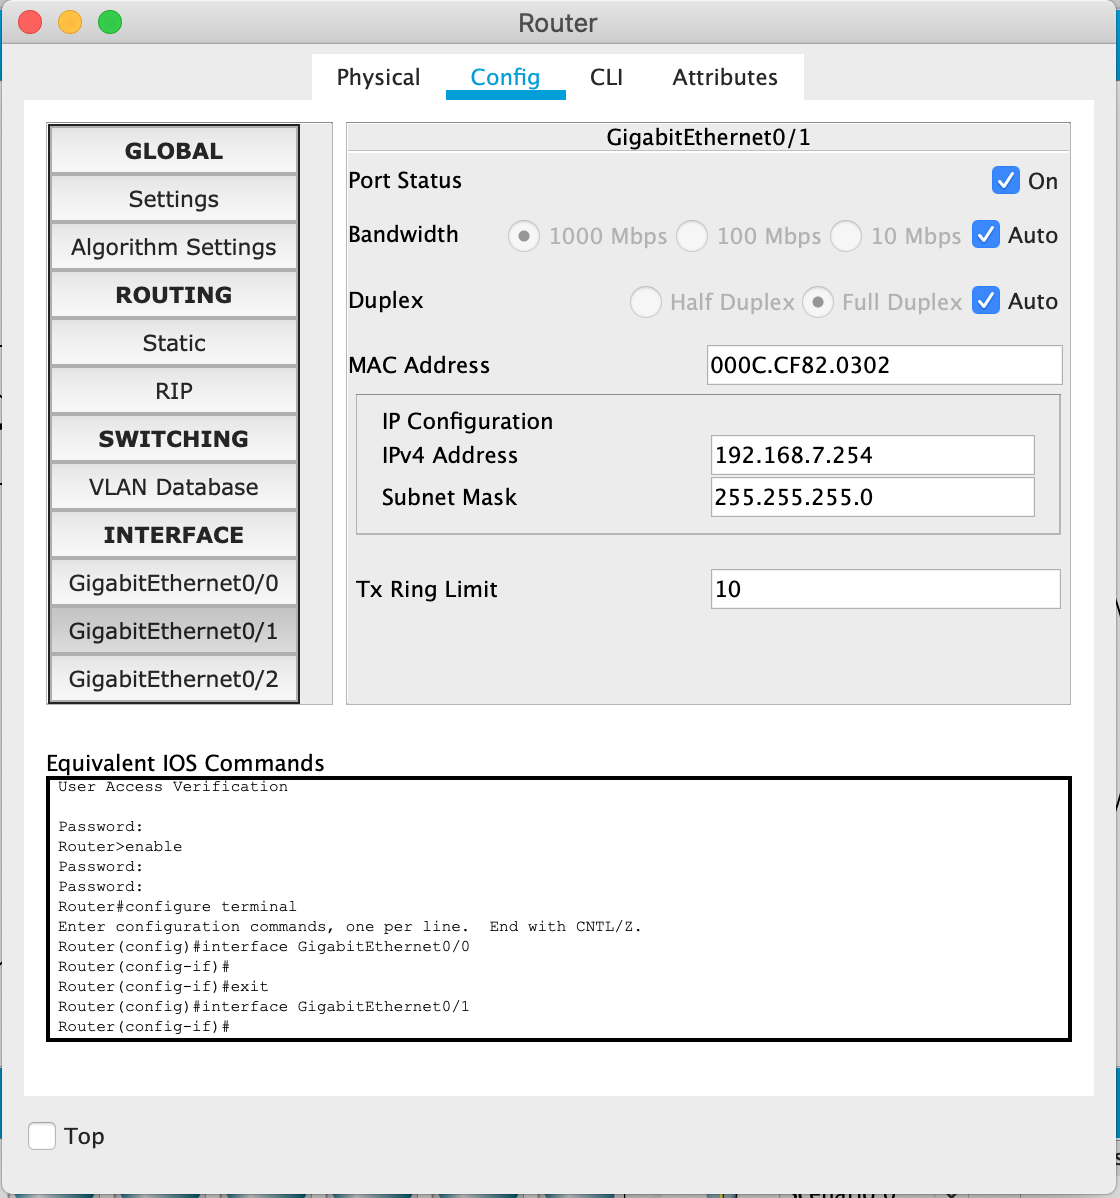
\includegraphics[width=\textwidth]{6.1.png}
		\end{minipage}
		\begin{minipage}[b]{0.32\textwidth}
			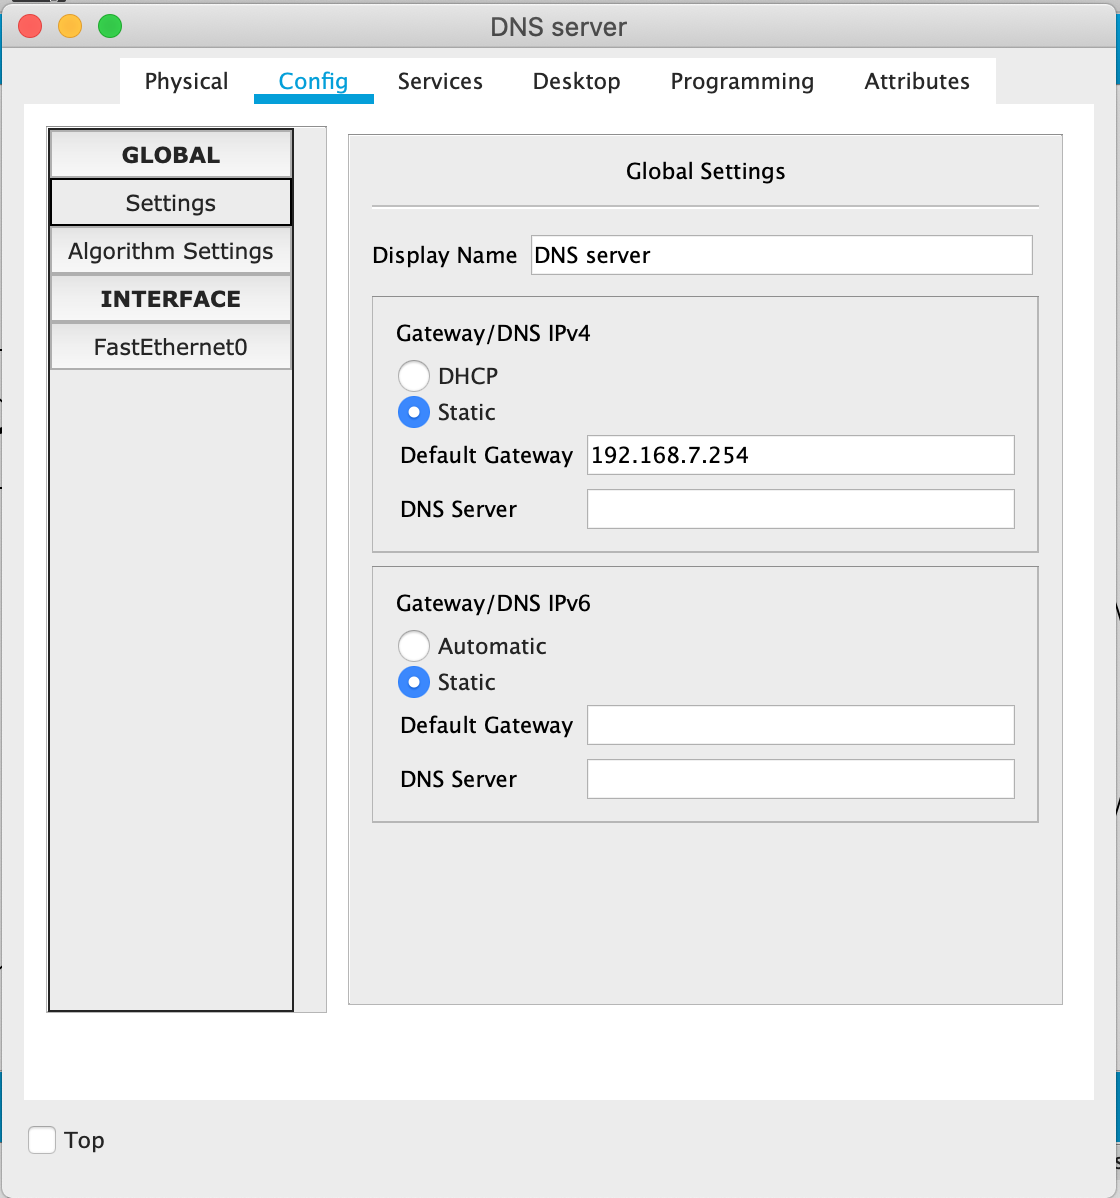
\includegraphics[width=\textwidth]{6.2.png}
		\end{minipage}
		\center{Установка портов маршрутизатора как адрес шлюза по умолчанию
			для конечных узлов (сеть 2)}
		\label{ris:6}
	\end{figure}

	\begin{figure}[h!]
		\begin{minipage}[b]{0.32\textwidth}
			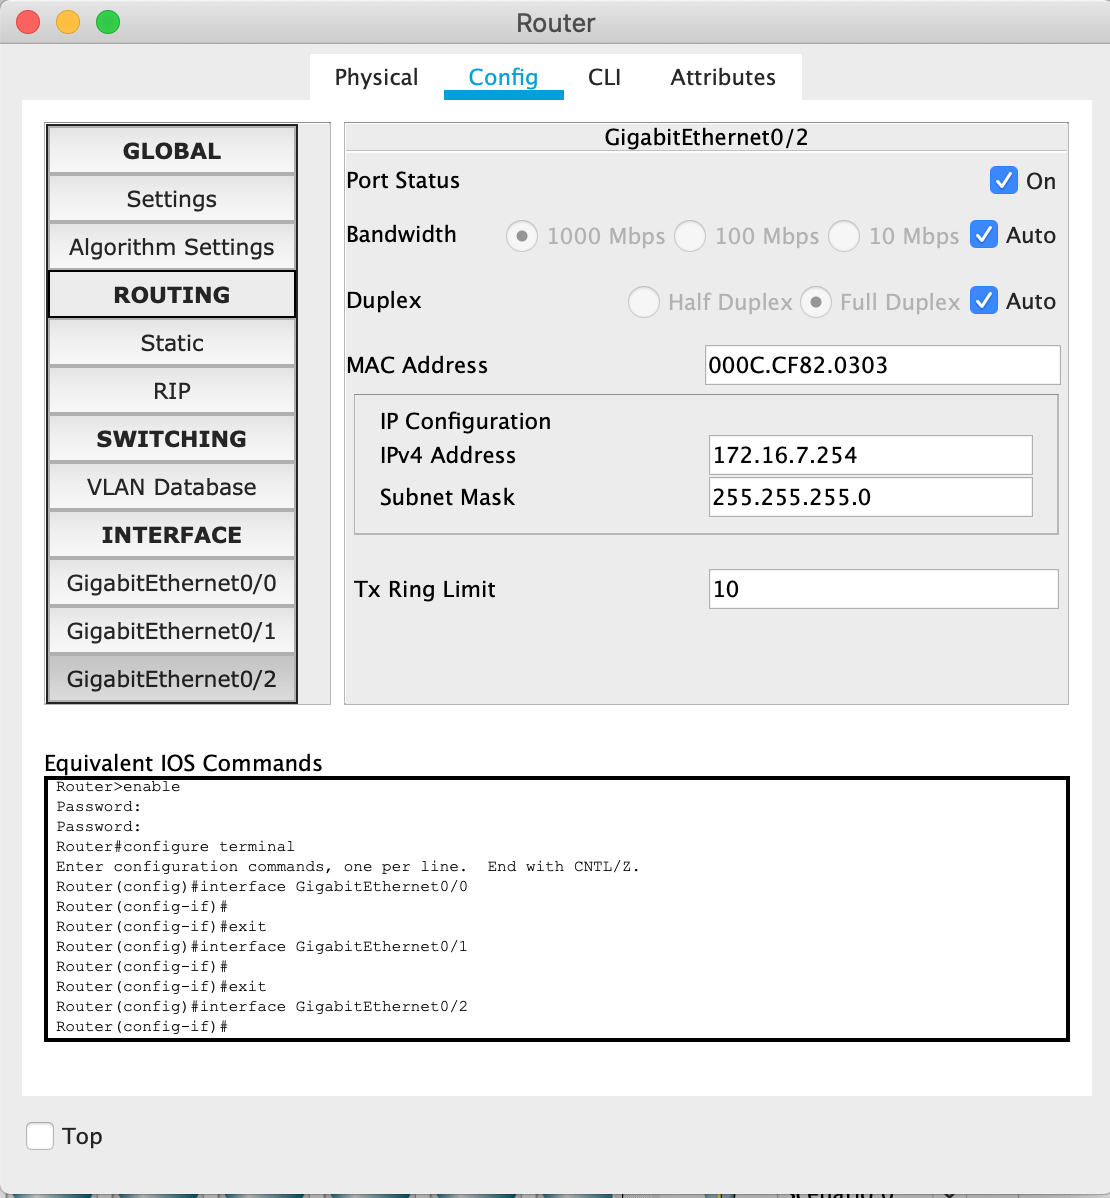
\includegraphics[width=\textwidth]{7.1.png}
		\end{minipage}
		\begin{minipage}[b]{0.32\textwidth}
			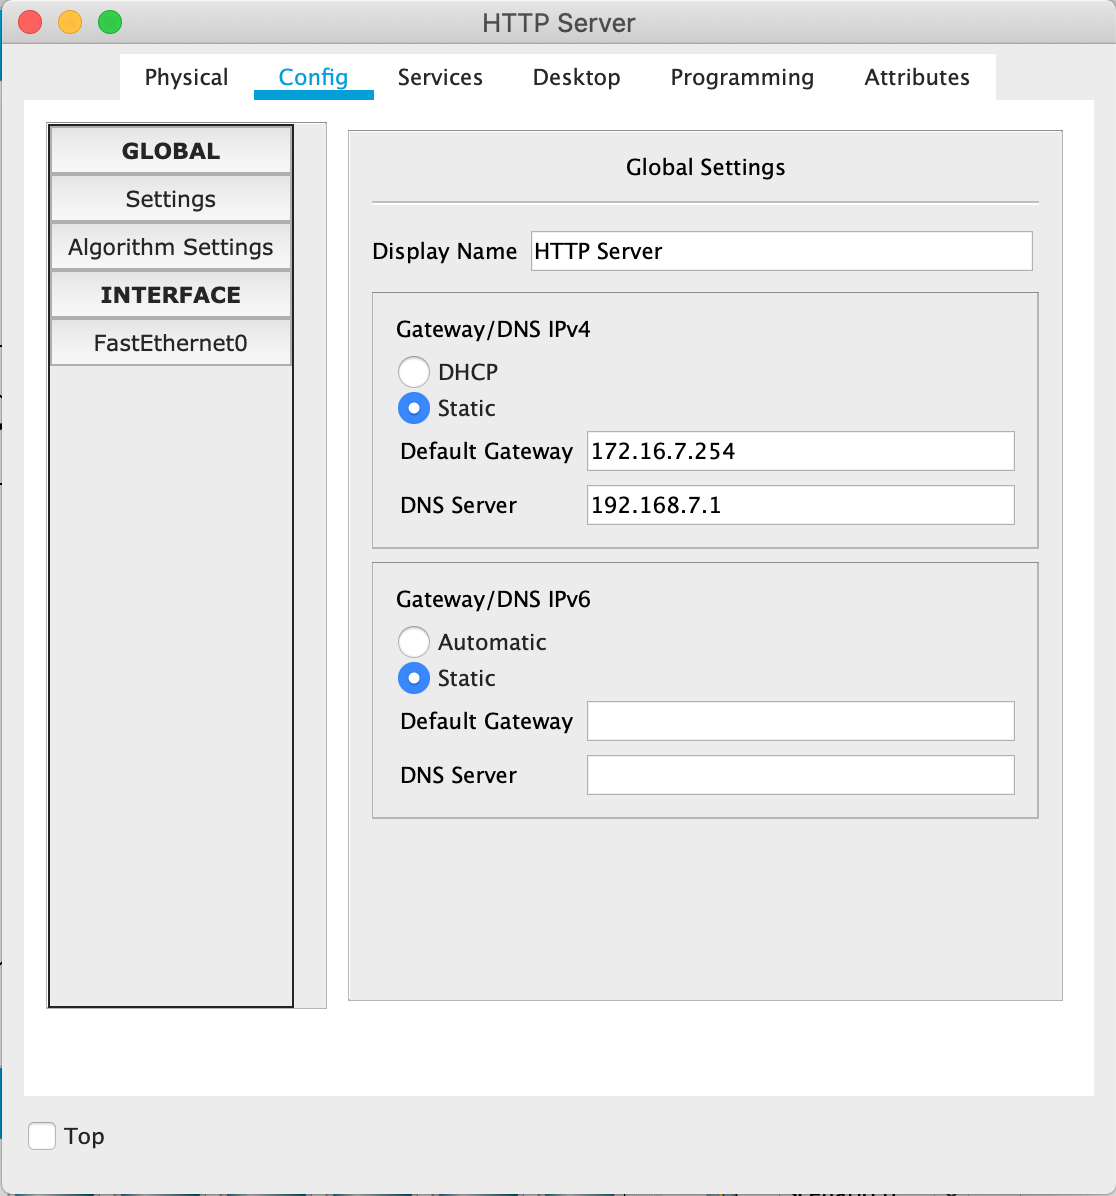
\includegraphics[width=\textwidth]{7.2.png}
		\end{minipage}
		\begin{minipage}[b]{0.32\textwidth}
			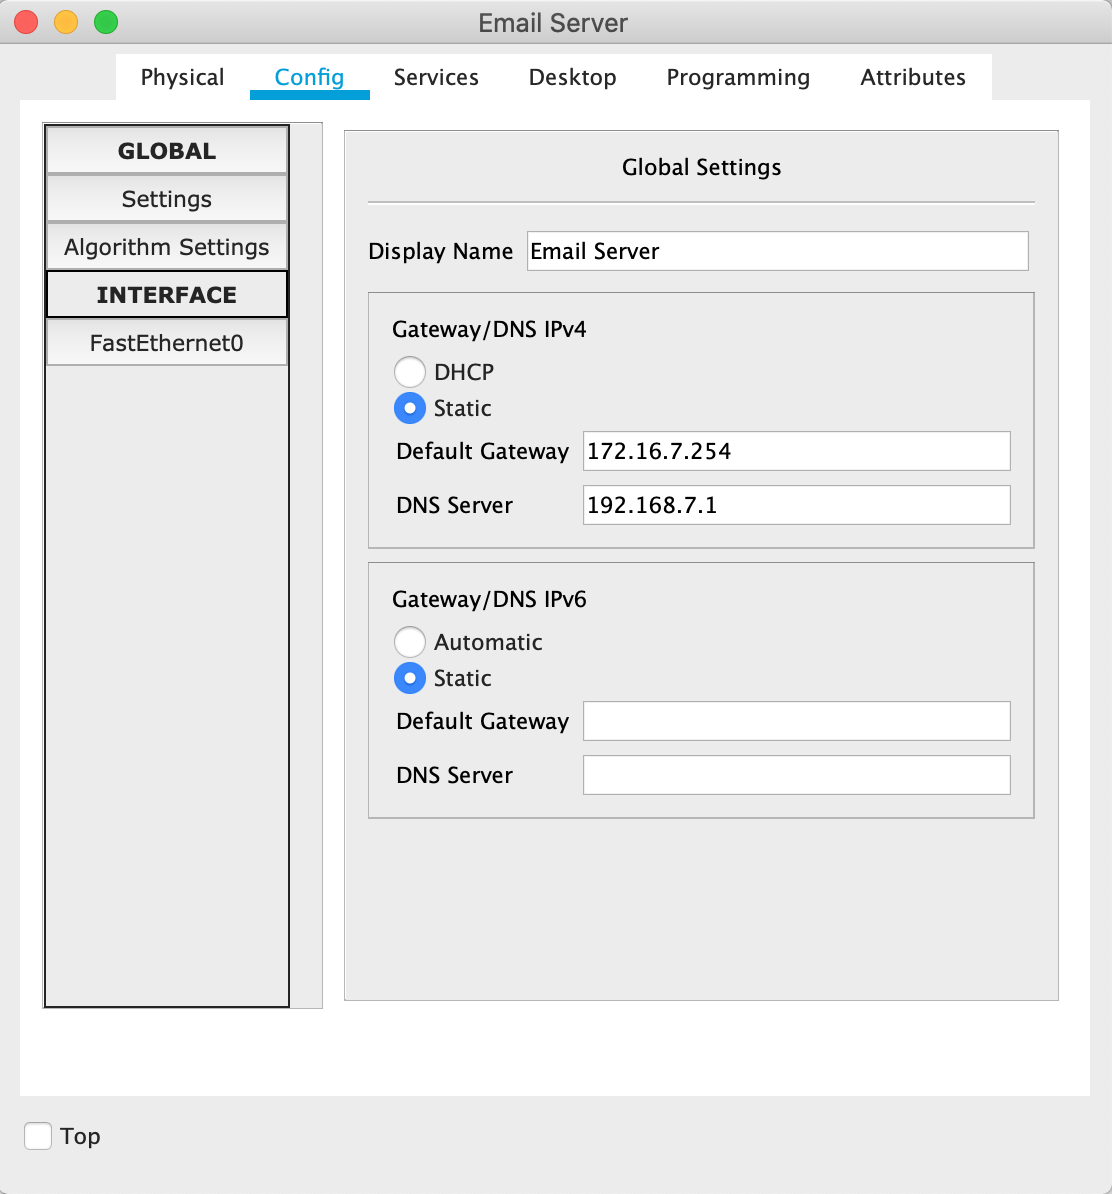
\includegraphics[width=\textwidth]{7.3.png}
		\end{minipage}
		\center{Установка портов маршрутизатора как адрес шлюза по умолчанию
			для конечных узлов (сеть 3)}
		\label{ris:7}
	\end{figure}

	\newpage

	\section{Настроить DNS-сервер. Добавить почтовые записи на DNS-сервер.}
	
	\begin{figure}[h!]
		\begin{center}
			{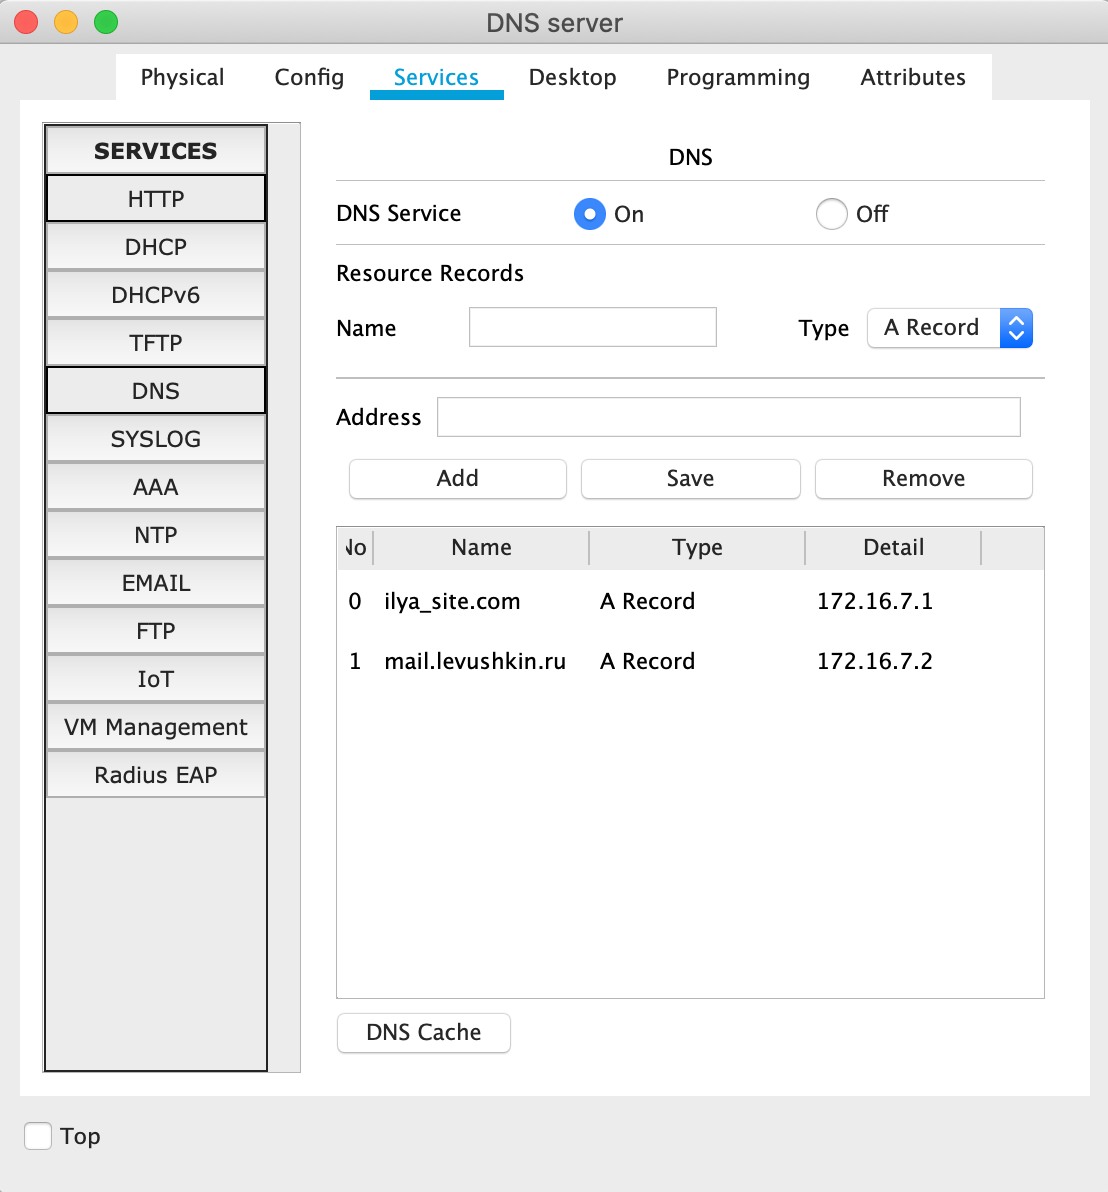
\includegraphics[scale = 0.7]{8.png}}
			\label{ris:8}
		\end{center}
		\caption{Настройка DNS-сервера}
	\end{figure}

	\newpage
	
	\section{Настроить почтовый сервер SMTP и POP3.}
	
	\begin{figure}[h!]
		\begin{center}
			{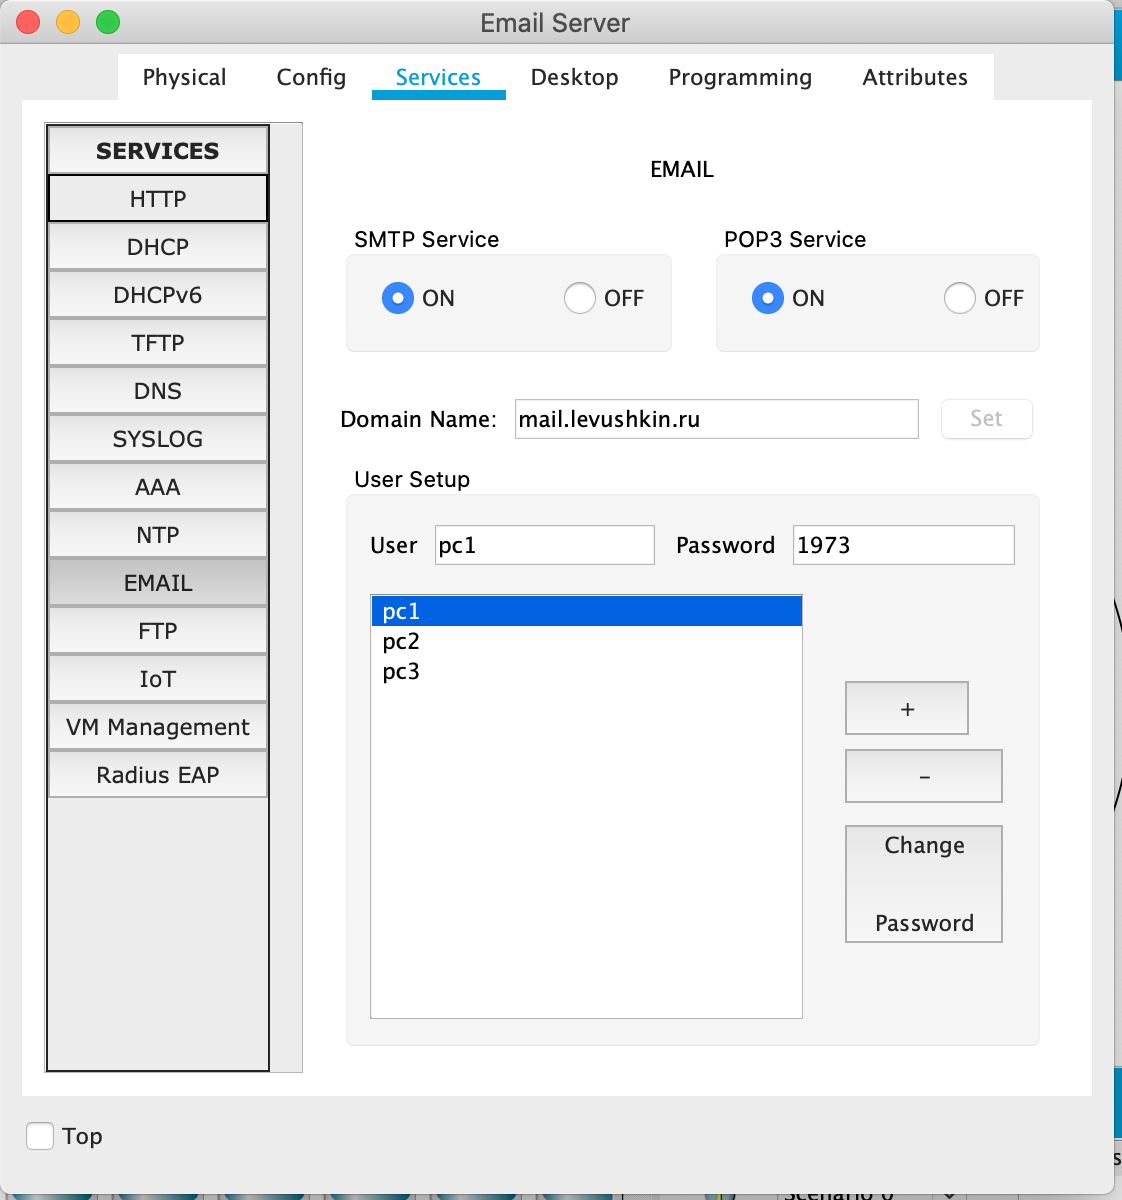
\includegraphics[scale = 0.7]{9.png}}
			\label{ris:9}
		\end{center}
		\caption{Настройка почтового сервера}
	\end{figure}

	\newpage
	
	\section{Настроить почтовый клиент на всех ПК.}
	
	\begin{figure}[h!]
		\begin{minipage}[b]{0.32\textwidth}
			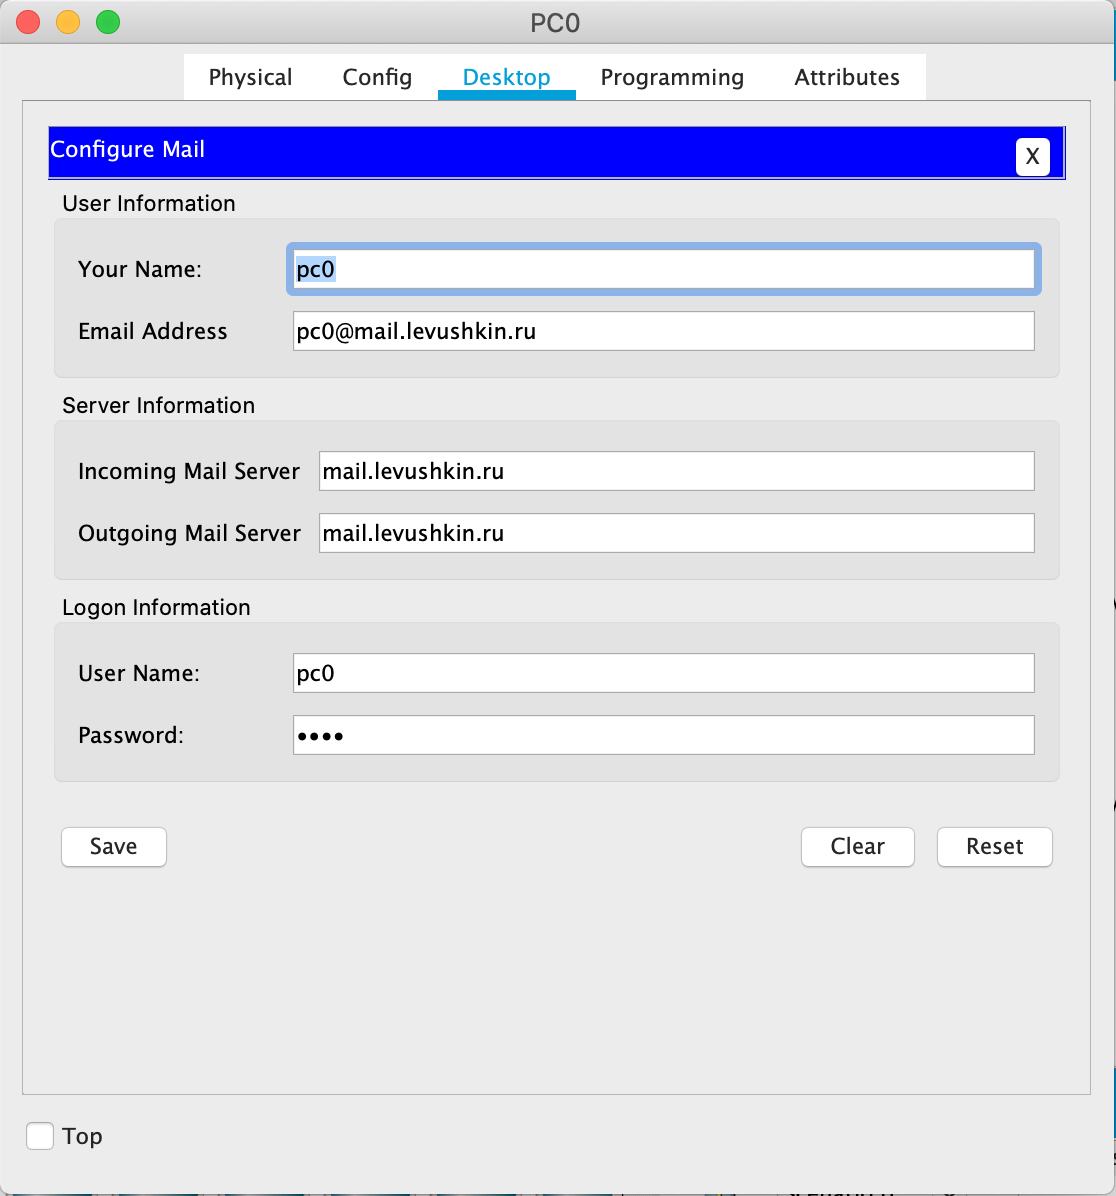
\includegraphics[width=\textwidth]{10.1.png}
		\end{minipage}
		\begin{minipage}[b]{0.32\textwidth}
			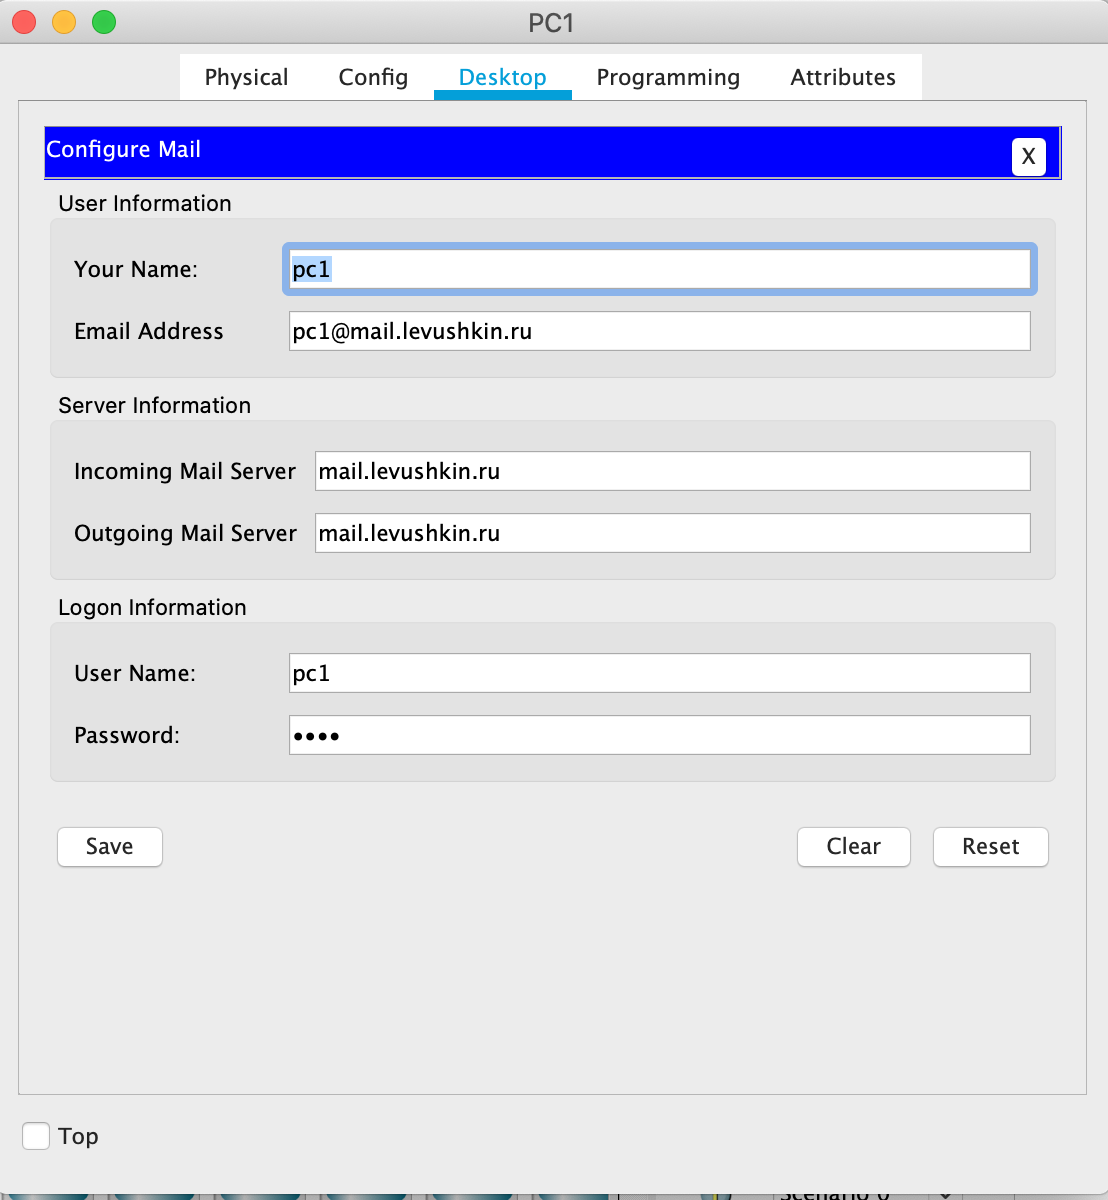
\includegraphics[width=\textwidth]{10.2.png}
		\end{minipage}
		\begin{minipage}[b]{0.32\textwidth}
			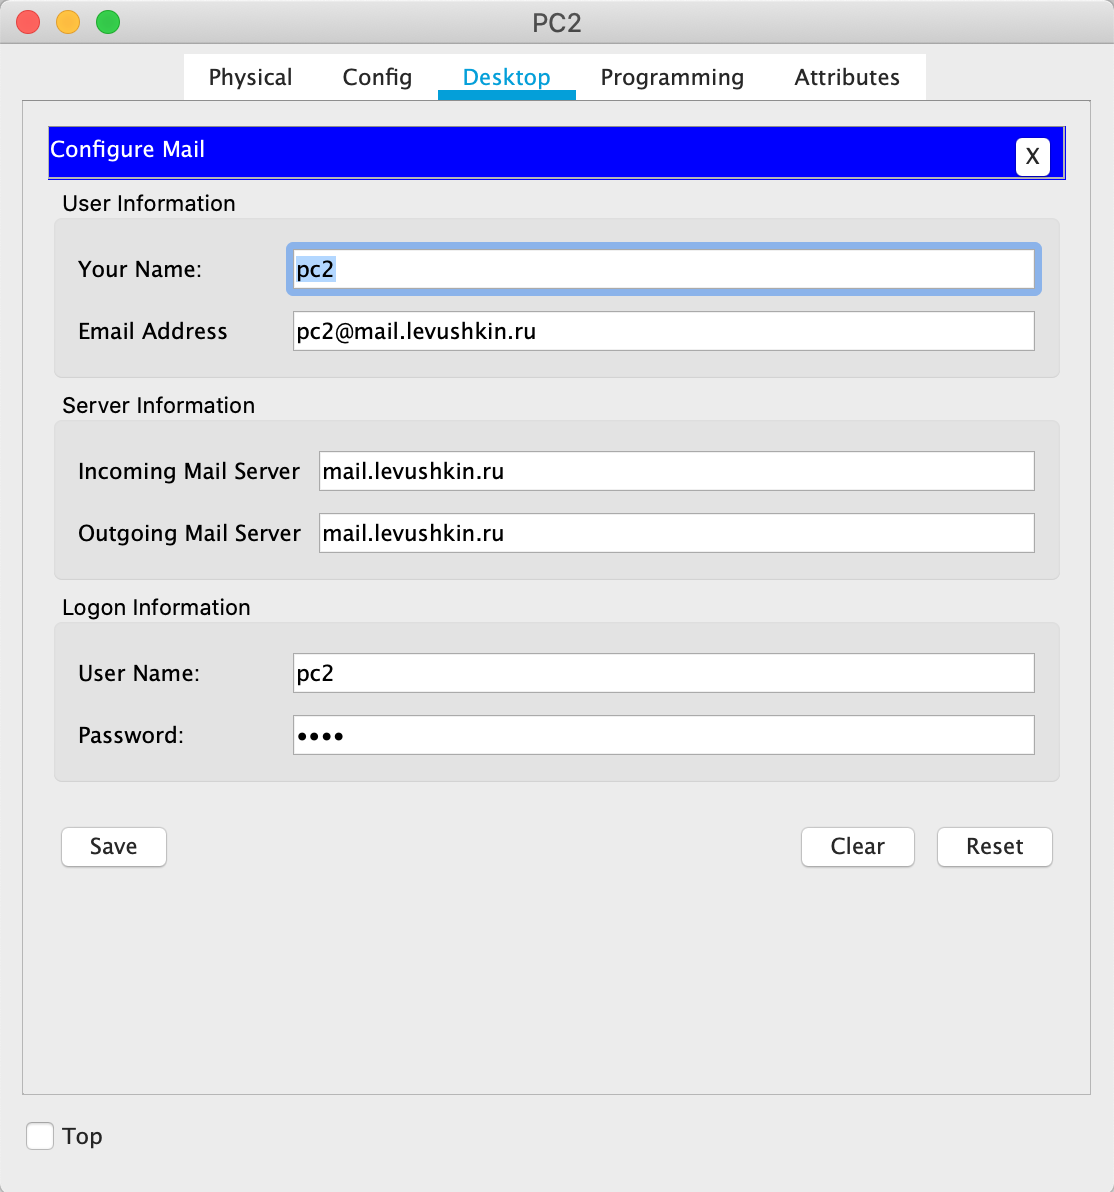
\includegraphics[width=\textwidth]{10.3.png}
		\end{minipage}
		\center{Настройка почтовых клиентов на ПК}
		\label{ris:10}
	\end{figure}

	\newpage
	
	\section{Настроить HTTP-сервер, разместить там тестовую страницу с номером варианта, фамилией, номером группы, датой выполнения работы.}
	
	\begin{figure}[h!]
		\begin{center}
			{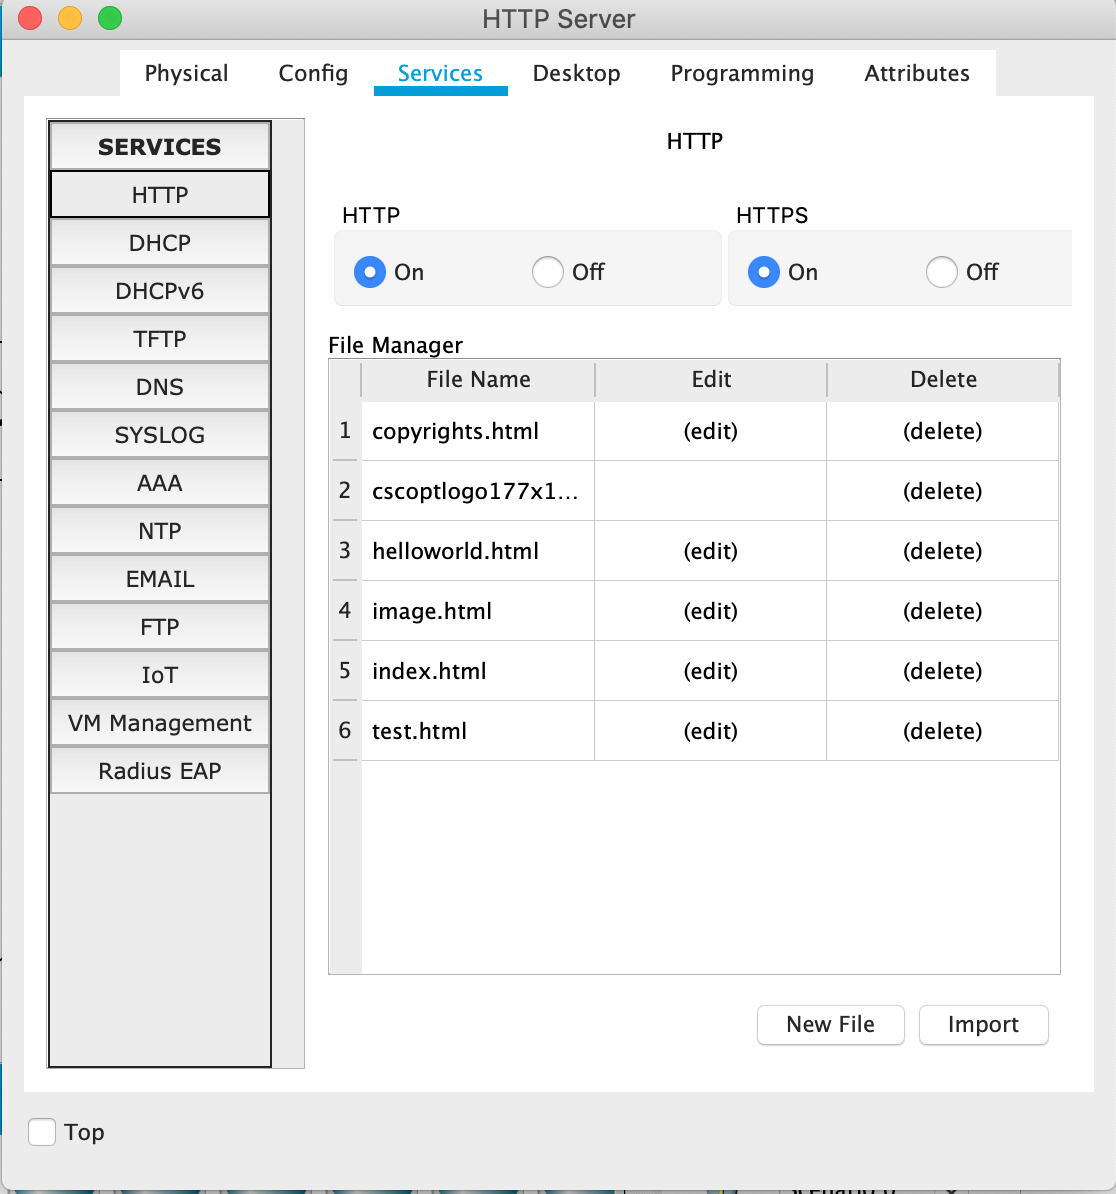
\includegraphics[scale = 0.45]{11.png}}
			\label{ris:11}
		\end{center}
		\caption{Настройка HTTP-сервера}
	\end{figure}

	\begin{figure}[h!]
		\begin{center}
			{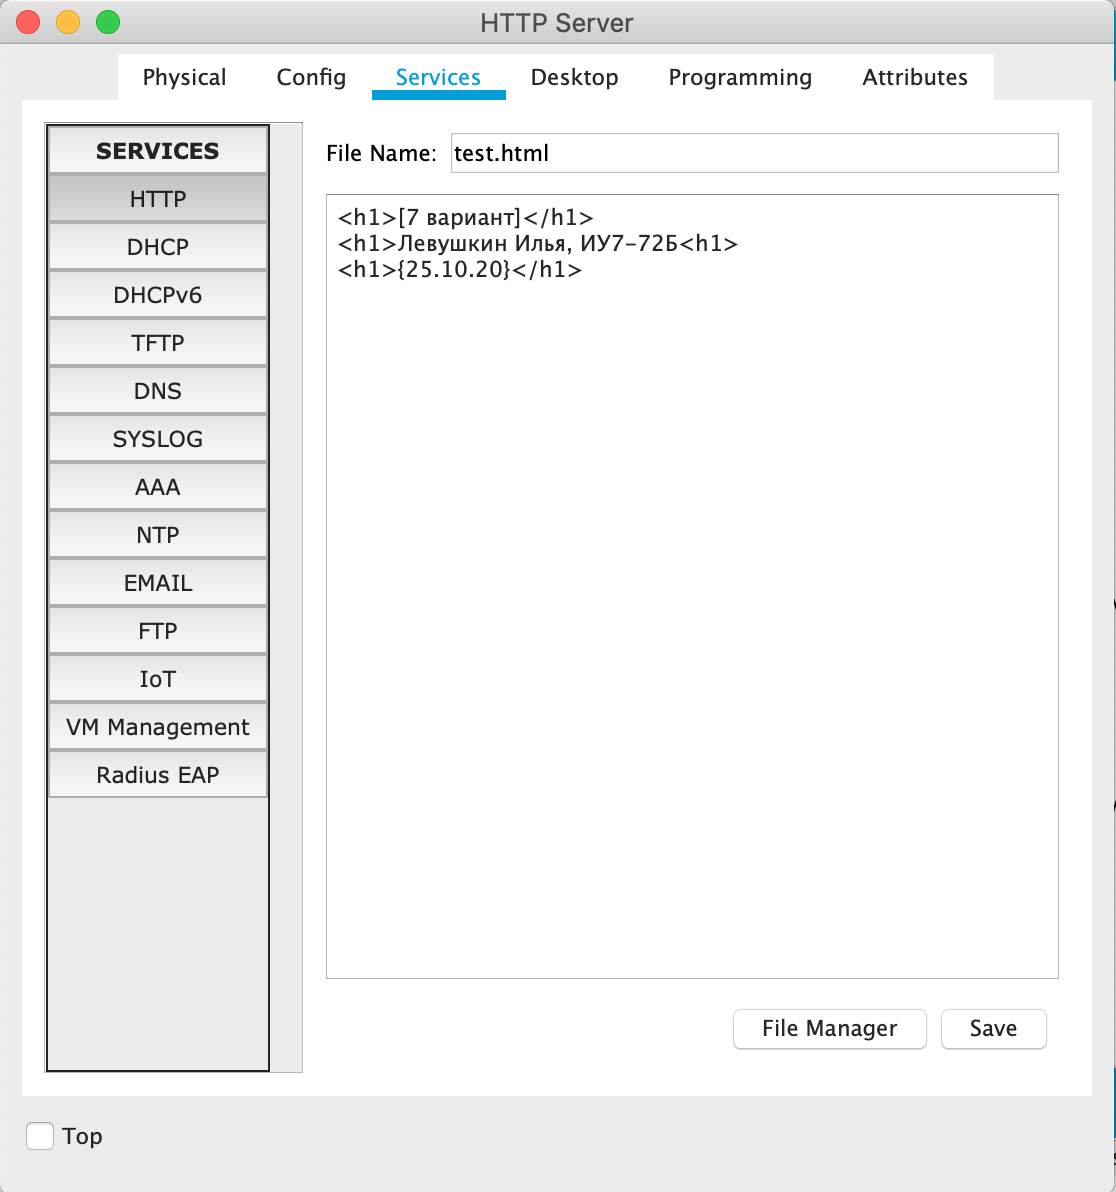
\includegraphics[scale = 0.45]{12.png}}
			\label{ris:12}
		\end{center}
		\caption{Тестовая страница}
	\end{figure}

	\newpage
	
	
	\section{Проверить корректное прохождение сигнала между всеми узлами сети, доступность настроенных сервисов со стороны клиентов на ПК.}
	
	\begin{figure}[h!]
		\begin{center}
			{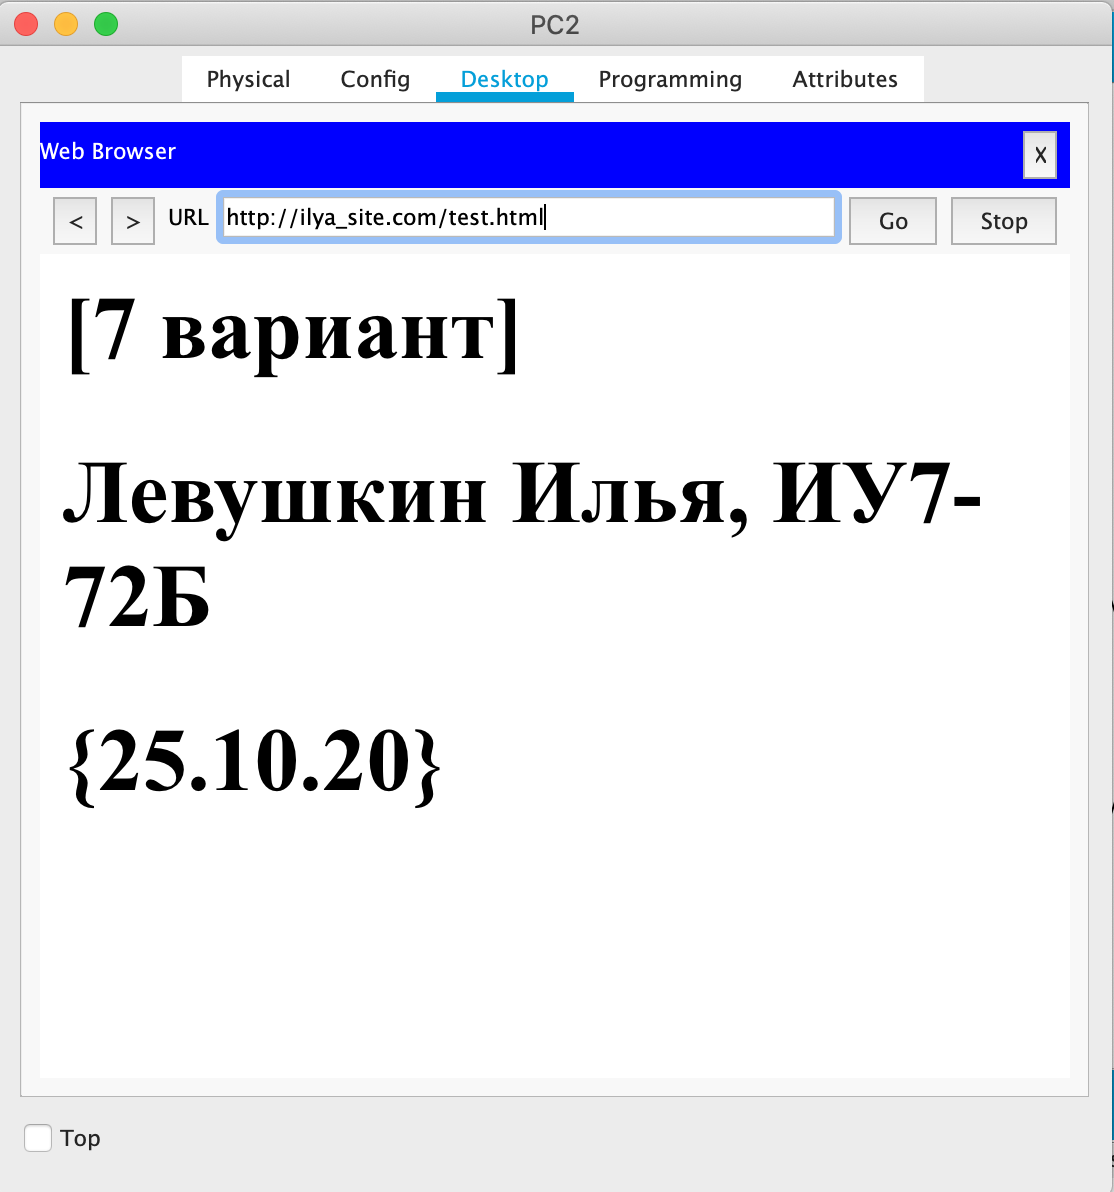
\includegraphics[scale = 0.45]{13.png}}
			\label{ris:13}
		\end{center}
		\caption{Проверка доступа к HTTP-серверу}
	\end{figure}

	\begin{figure}[h!]
		\begin{center}
			{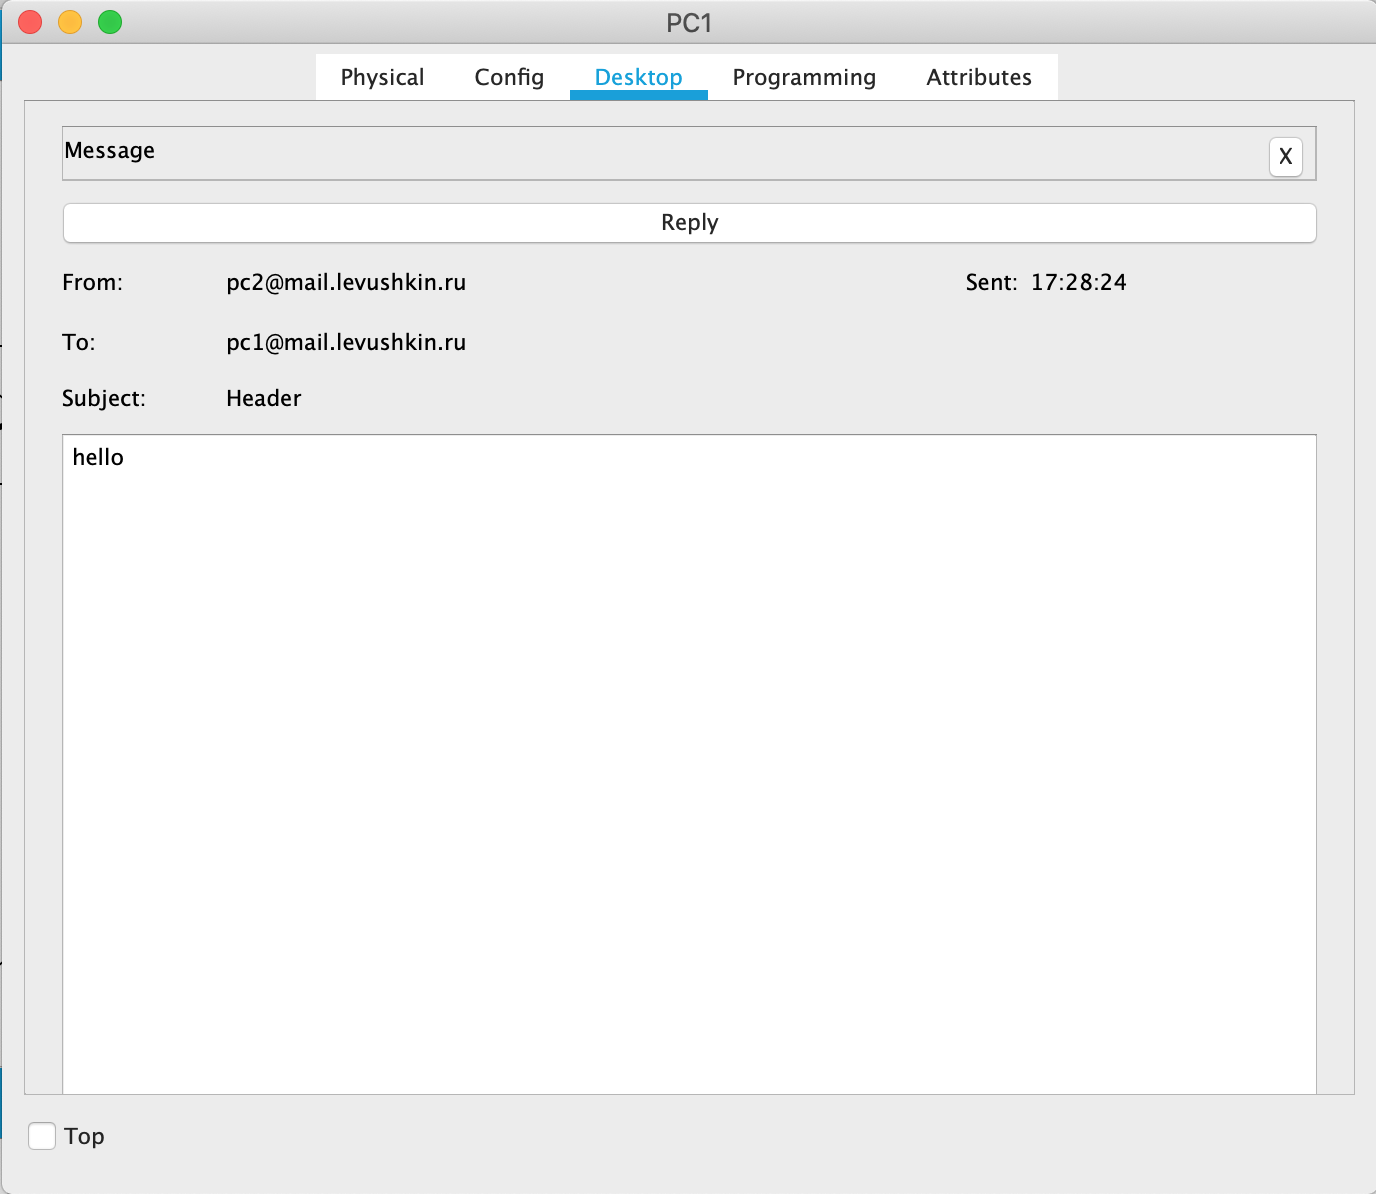
\includegraphics[scale = 0.45]{14.png}}
			\label{ris:14}
		\end{center}
		\caption{Проверка работоспособности почтового сервиса}
	\end{figure}
	
	\section{Отметить широковещательные домены и домены коллизий на схеме.}
	
	\begin{figure}[h!]
		\begin{center}
			{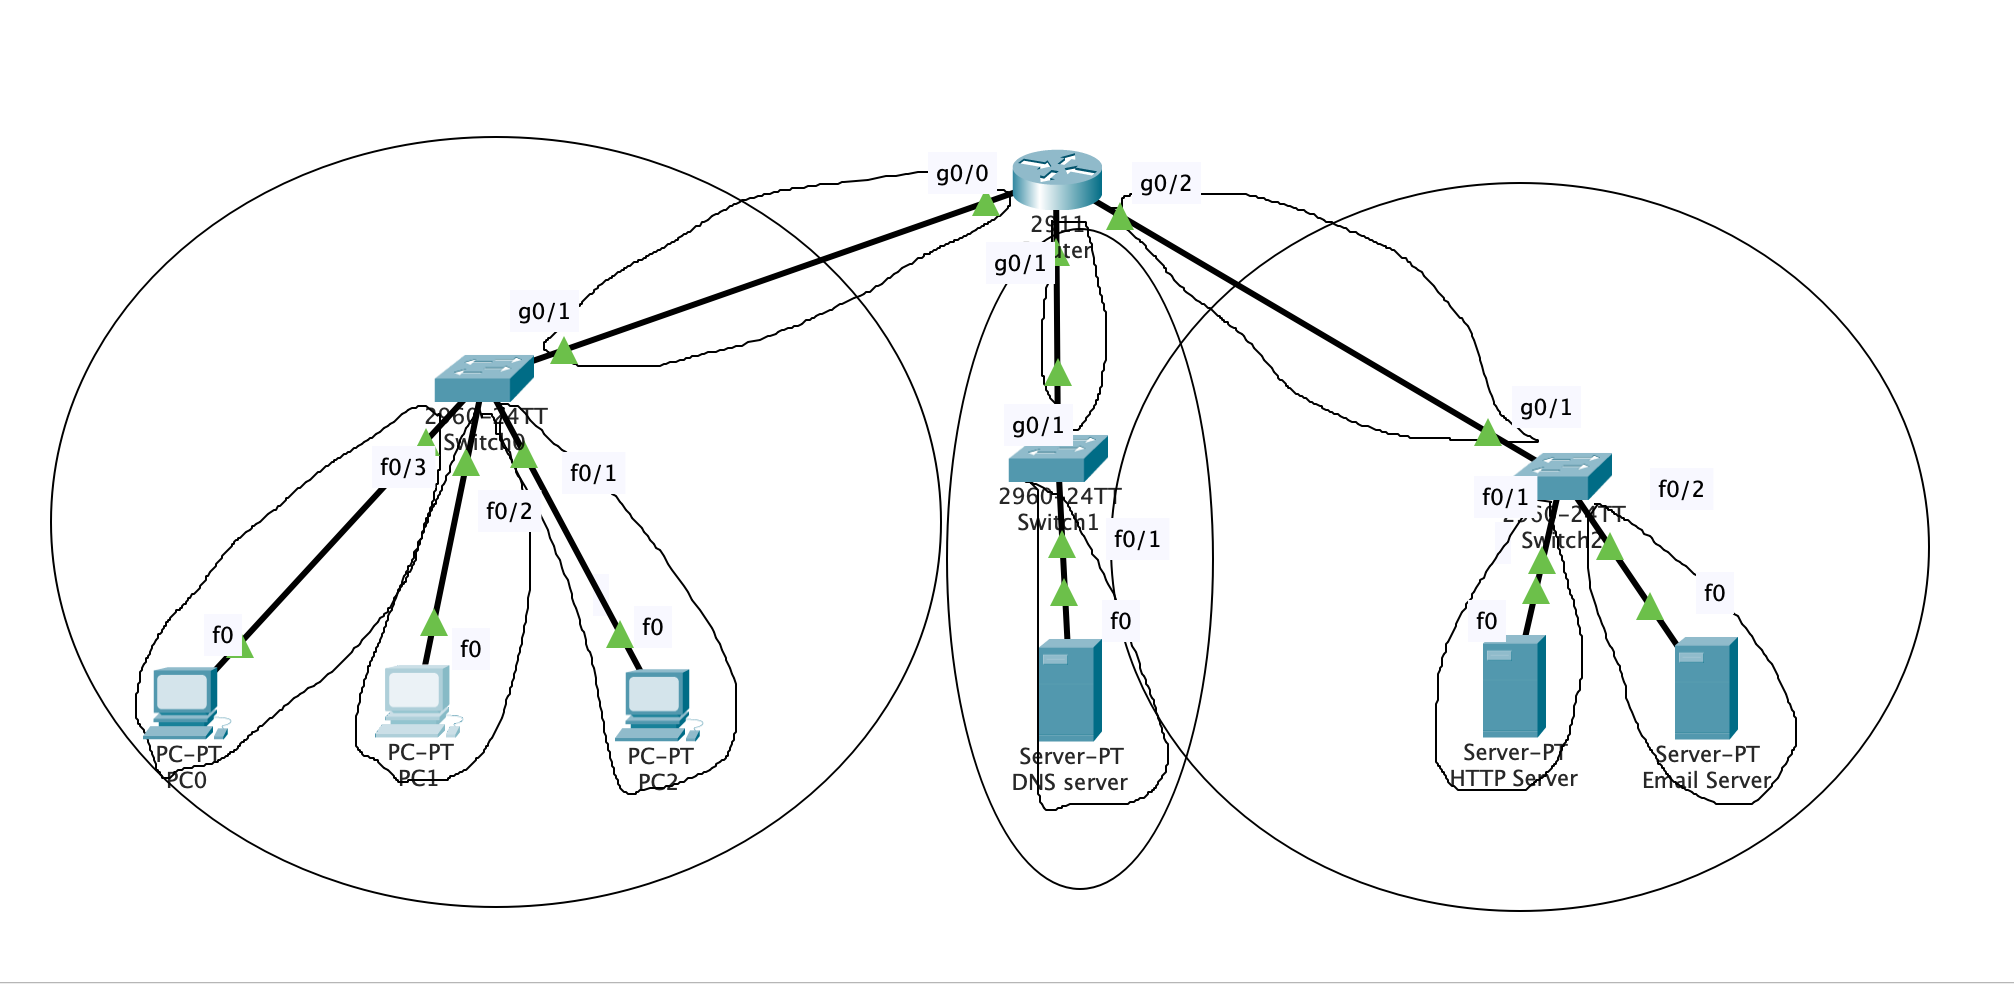
\includegraphics[scale = 0.5]{15.png}}
			\label{ris:15}
		\end{center}
		\caption{Широковещательные домены – круги; домены
			коллизий – овалообразные фигуры}
	\end{figure}
	
\end{document}